\section{Evklidske in origami konstrukcije}
\label{pogl:aksiomi}

Kraj in čas izvora origamija nista jasno določena. Nekateri viri zatrjujejo, da izhaja iz Japonske, drugi ga pripisujejo Kitajski, tretji se ne strinjajo z nobeno od teh dveh možnosti. Verjetno so umetnost zlaganja odkrili še pred izumom papirja, za katerega je leta 105 po Kr. poskrbel kitajski dvorni uradnik Cai Lun, saj se da npr.\ zlagati tudi robce iz blaga~\cite{robinson2024}. Je pa papir idealen material za zlaganje. Japonska beseda \emph{origami} kot umetnost zgibanja papirja (``oru'' -- prepogibati, ``kami'' -- papir) se je na Daljnem vzhodu začela uporabljati proti koncu 19. stoletja.

Povečano zanimanje za origami v matematiki se je začelo v 2.\ pol.\ 20.\ stoletja in s seboj prineslo množično izhajanje literature o povezavi origamija z matematiko, fiziko, astronomijo, računalništvom, kemijo in še mnogimi drugimi vedami~\cite{zore2022}. V angleščini je tako za matematično raziskovanje s prepogibanjem papirja nastalo poimenovanje ``\emph{origamics}''. V slovenščini uradnega prevoda še ni, Grahor pa v~\cite[str.\ 5]{sgv2016} po zgledu angleških poimenovanj nekaterih znanstvenih disciplin (\emph{mathematics} -- matematika, \emph{physics} -- fizika itd.) predlaga termin ``origamika''.

\subsection{Evklidovi postulati in evklidske konstrukcije}

Preden si pogledamo, kaj lahko s prepogibanjem papirja konstruiramo, se spomnimo, na čem temelji evklidska geometrija. Za njenega očeta štejemo grškega matematika Evklida\footnote{O življenju tega aleksandrijskega učenjaka ne vemo nič gotovega, je pa zelo verjetno živel za časa prvega Ptolemaja (faraon v času 306--283 pr.\ Kr.)~\cite[str.\ 61]{struik1986}.}, ki je napisal zelo znano zbirko trinajstih knjig pod skupnim imenom \emph{Elementi}. V njih obravnavana snov temelji na strogo logični izpeljavi izrekov iz definicij%\footnote{\emph{Definicija} je nedvoumno jasna opredelitev novega pojma.}
, aksiomov in postulatov\footnote{\emph{Aksiom} je temeljna resnica ali načelo, ki ne potrebuje dokazov (oz.\ dokaz sploh ne obstaja) in vedno velja. \emph{Postulat} je predpostavka oz.\ zahteva. Evklid med aksiomi in postulati ni postavil jasne razlike, Aristotel pa je postulat od aksioma ločil po tem, da gre pri prvem bolj za hipotezo kot temeljno resnico, vendar se njene veljavnosti ne dokazuje, temveč privzame kot veljavno~\cite[str.\ 122]{euclidI}. V primeru petega Evklidovega postulata se bomo spomnili, da nam to, ali ga privzamemo ali ne, poda različne geometrije. Danes med pojmoma ne ločujemo~\cite[str.\ 2]{geometricconstructions}.}. Še danes večina osnovno- in srednješolske geometrije izvira prav iz prvih šestih knjig Elementov.

V prvi knjigi Elementov je Evklid najprej definiral osnovne pojme -- točka, premica, površina, ravnina, ravninski kot, pravi kot, ostri kot, topi kot, krog, središče kroga, premer, enakostranični in enakokraki trikotnik, kvadrat \ldots ter nazadnje upeljal še pojem vzporednih premic~\cite{euclidI}. Nato je zapisal znamenitih pet postulatov, iz katerih izhaja vsa evklidska geometrija:

\renewcommand{\thepostulat}{P\arabic{postulat}}

\begin{postulat}
    \label{post:P1}
    Med dvema poljubnima točkama je mogoče narisati ravno črto.
\end{postulat}
\begin{postulat}
    \label{post:P2}
    Vsako ravno črto je mogoče na obeh koncih podaljšati.
\end{postulat}
\begin{postulat}
    \label{post:P3}
    Mogoče je narisati krožnico s poljubnim središčem in poljubnim polmerom.
\end{postulat}
\begin{postulat}
    \label{post:P4}
    Vsi pravi koti so med seboj skladni.
\end{postulat}
\begin{postulat}
    \label{post:P5}
    Če poljubni ravni črti sekamo s tretjo ravno črto (prečnico) in je vsota notranjih kotov na eni strani prečnice manjša od vsote dveh pravih kotov, potem se dani premici, če ju dovolj podaljšamo, sekata na tej strani prečnice.
    \opomba{Vemo že, da je postulat~\ref{post:P5} ekvivalenten \emph{aksiomu o vzporednicah}, ki pravi, da skozi dano točko, ki ne leži na dani premici, poteka natanko ena vzporednica k tej premici. Če ga predpostavimo, dobimo evklidsko geometrijo, sicer pa obstajajo še druge geometrije (npr.\ hiperbolična in sferna geometrija).}
\end{postulat}

\begin{definicija}
    \label{def:evklidske_konstrukcije}
    \emph{Evklidske konstrukcije} so konstrukcije točk, daljic, poltrakov, premic, krožnih lokov in krožnic, ki jih je iz danih točk in razdalj mogoče konstruirati le z uporabo t.~i.\ \emph{evklidskega orodja} -- neoznačenega in neskončno dolgega ravnila (angl.\ \emph{straightedge}) ter šestila, ki ne prenaša razdalj (ko ga dvignemo od podlage, se njegova kraka zložita skupaj). Vsak korak konstrukcije izhaja iz zgornjih postulatov in je lahko eden od naslednjih postopkov:
    \begin{itemize}
        \item risanje premice skozi dve dani točki,
        \item risanje krožnice s središčem v dani točki, ki poteka skozi drugo dano točko,
        \item določitev nove točke kot presečišče dveh danih premic, dveh danih krožnic ali danih premice in krožnice.
    \end{itemize}
\end{definicija}

\begin{opomba}
    \label{opom:solsko_sestilo}
    Da se pokazati, da lahko za konstrukcije ekvivalentno uporabimo tudi šestilo, ki prenaša razdalje~\cite[str.\ 6--7]{geometricconstructions}. Zato imamo odslej z izrazom \emph{šestilo} v mislih kar moderno šolsko šestilo.
\end{opomba}

Izkaže se, da z evklidskim orodjem ne moremo izvesti poljubnih konstrukcij -- kot zelo znane protiprimere lahko tu naštejemo tri starogrške probleme. Pri \emph{kvadraturi kroga} nam evklidsko orodje ne zmore konstruirati razdalje $\sqrt{\pi}$, pri \emph{podvojitvi kocke} razdalje $\sqrt[3]{2}$, pri \emph{trisekciji kota} ne zmore poljubnega kota razdeliti na tri enake dele. Drugi in tretji problem sta, verjetno za marsikoga presenetljivo, rešljiva z origamijem. V poglavju~\ref{pogl:starogrskiproblemi} si bomo pogledali njuni rešitvi, sedaj pa podrobneje spoznajmo še konstrukcije, ki jih dobimo s prepogibanjem papirja.

\subsection{Origami konstrukcije}
\label{origami_konstrukcije}

V nalogi se bomo omejili le na prepogibanje v ravnini in se z trodimenzionalni modeli ne bomo ukvarjali. Bralec je ob branju povabljen, da opisane konstrukcije v praksi preizkusi tudi sam. Pri izbiri papirja je priporočljiv rahlo prosojen papir, skozi katerega se vidijo morebitne označbe točk in premic s svinčnikom (npr.\ navaden kuhinjski papir za peko).

Bistvo origamija je, da prepogibamo list papirja. Zato je tudi naravno, da ga vzamemo za model evklidske ravnine. V njej si za modele premic vzamemo \emph{ravne} pregibe, modeli točk pa naj bodo presečišča premic, tj.\ \emph{presečišča pregibov}. Določimo še nekaj pravil:
\begin{itemize}
    \item pregibe opravljamo \emph{po enega naenkrat}, torej po vsakem pregibu papir nazaj razgrnemo,
    \item ne uporabljamo drugih orodij, kot so ravnilo, šestilo, škarje, lepilo ipd.,
    \item pisalo je dovoljeno le pogojno -- z njim lahko označimo pomožne točke, za katere vemo, da jih znamo konstruirati z origamijem, ampak bi nam pomožni pregibi zmanjšali preglednost konstrukcije (npr.\ zrcaljene točke, glej razdelek~\ref{podpogl:zrcaljenje_origami}); prav tako lahko s pomočjo ravnila močneje poudarimo že konstruirane točke in premice.
\end{itemize}

Papir prepogibamo tako, da se objekti na njem (točke in premice) prekrijejo. Zato moramo na začetku imeti na listu že nekaj danih objektov (npr.\ dve različni točki ali premico in točko, ki ne leži na njej). Hull v~\cite[str.\ 24--26]{hull2020} navaja spodnji seznam vseh mogočih pregibov (po vrsti so prikazani na sliki~\ref{fig:vsi_pregibi}):
\begin{itemize}
    \item točko prepognemo na drugo točko (en možen pregib),
    \item točko prepognemo samo vase (neskončno možnih pregibov),
    \item točko prepognemo na premico (neskončno možnih pregibov),
    \item premico prepognemo na drugo premico (en ali dva možna pregiba) in
    \item premico prepognemo samo vase (neskončno možnih pregibov).
\end{itemize}

\begin{figure}[h]
    \centering
    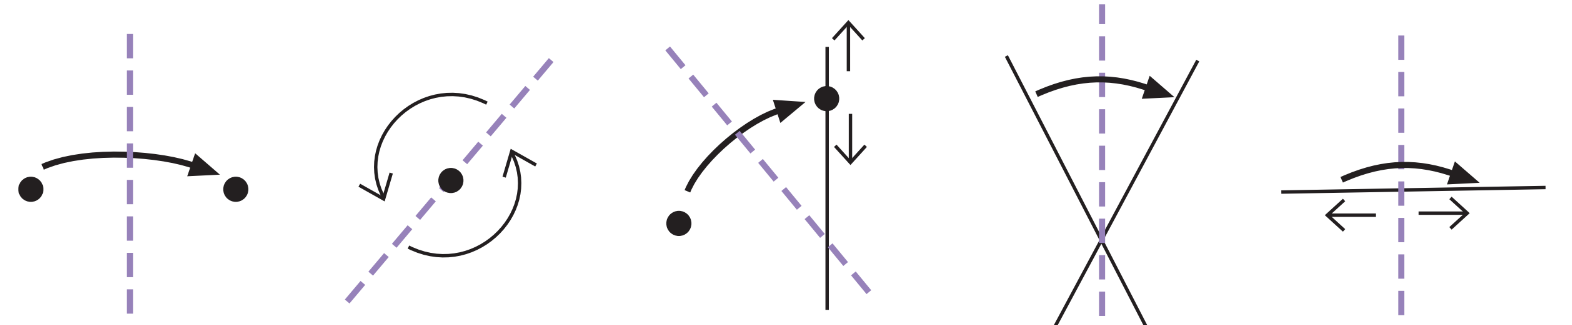
\includegraphics[width=0.8\textwidth]{images/hull_vsi pregibi.png}
    \caption[Vsi mogoči pregibi]{Vsi pregibi točk ali premic na točko ali premico. Vzeto iz~\cite[str.\ 25]{hull2020}.}
    \label{fig:vsi_pregibi}
\end{figure}

Vidimo lahko, da je pri nekaterih primerih pregibov neskončno možno in tega si ne želimo. Tako kot pri evklidskih konstrukcijah na primer ne dovolimo konstrukcij premic, ki potekajo skozi eno samo točko (šop premic), bomo tudi tu možne pregibe omejili na končno število možnosti. V ta namen sedaj definirajmo vse možne pregibe.

\subsubsection{Origami operacije in origami konstrukcije}
\label{podpodpogl:operacije}

V zadnjem stoletju se je preko več matematikov (Jacques Justin, Peter Messer, Benedetto Scimemi, Humiaki Huzita, Koshiro Hatori, George E.\ Martin idr.; nekateri so med seboj sodelovali, drugi so delovali neodvisno) skozi čas izoblikoval seznam t.~i.\ \emph{origami operacij}. Gre za nekakšne ``aksiome''\footnote{Seznam je bolj znan pod imenom \emph{Huzita-Hatori aksiomi}, vendar izraz ``aksiom'' tu ni primeren, saj bomo kmalu pokazali, da se med seboj prepletajo in so nekateri izmed njih kombinacija drugih. Prav tako v tej nalogi v ime seznama ne vključimo imen avtorjev, ker se svoj del k seznamu prispevalo več drugih avtorjev.} o obstoju specifičnih prepogibov, ki zajamejo vseh pet možnosti prepogibanja iz zgornjega Hullovega seznama. Da so to zadostne operacije za katerokoli origami konstrukcijo, si bomo pogledali v razdelku~\ref{podpogl:zadost_potr_op}.

Seznam se je med avtorji razlikoval v številu (gl.\ \cite[str.\ 29--30]{hull2020}), kot končen seznam pa bomo tu navedli vseh osem naštetih -- na prvi pogled različnih -- operacij. Najprej jih naštejmo, potem pa si ob sledečih slikah še natančneje poglejmo konstrukcijo in pomen posamezne operacije. Videli bomo, da moramo pri nekaterih operacijah ločiti več primerov~\cite{michael2005, zore2022}. Pregibi so na slikovnih prikazih označeni z rdečo prekinjeno črto.

\renewcommand{\theoperacija}{O\arabic{operacija}}

\begin{operacija}
    \label{op:O1}
    Za poljubni točki $A$ in $B$ obstaja natanko en pregib $p$, ki gre skoznju.
\end{operacija}
\begin{operacija}
    \label{op:O2}
    Za poljubni premici lahko določimo njuno presečišče, če obstaja.
\end{operacija}
\begin{operacija}
    \label{op:O3}
    Za poljubni točki $A$ in $B$ obstaja natanko en pregib $p$, da se točki pokrijeta.
\end{operacija}
\begin{operacija}
    \label{op:O4}
    Za poljubni premici $a$ in $b$ obstaja pregib $p$, ki ju položi eno na drugo.
\end{operacija}
\begin{operacija}
    \label{op:O5}
    Za poljubno točko $A$ in premico $a$ obstaja natanko en pregib $p$ skozi točko $A$, ki je pravokoten na premico $a$.
\end{operacija}
\begin{operacija}
    \label{op:O6}
    Za primerno izbrani točki $A$ in $B$ ter premico $a$ obstaja pregib $p$ skozi točko $B$, ki točko $A$ položi na premico $a$.
\end{operacija}
\begin{operacija}
    \label{op:O7}
    Za primerno izbrani točki $A$ in $B$ ter premici $a$ in $b$ obstaja pregib $p$, ki točko $A$ položi na premico $a$ in točko $B$ na premico $b$.
\end{operacija}
\begin{operacija}
    \label{op:O8}
    Za poljubno točko $A$ ter nevzporedni premici $a$ in $b$ obstaja pregib $p$, ki je pravokoten na premico $b$ in točko $A$ položi na premico $a$.
\end{operacija}

Vse operacije nam konstruirajo raven pregib (premico), le operacija~\ref{op:O2} nam določa njihova presečišča (točke). Iz tu lahko smiselno definiramo origami konstrukcije.

\begin{definicija}
    \label{def:origami_konstruktibilnost}
    \emph{Origami konstrukcije} so konstrukcije točk in premic, ki jih je iz danih točk in razdalj mogoče konstruirati preko operacij~\ref{op:O1}--\ref{op:O8}. Pri tem premico predstavlja raven in enkraten pregib iz posamezne operacije, nove točke pa so določene s presečišči teh pregibov.
\end{definicija}

Prve tri operacije so prikazane na sliki~\ref{fig:O1-O3}. Operacijo~\ref{op:O1} izvedemo tako, da naredimo pregib skozi točki $A$ in $B$. Takoj opazimo, da je ta operacija analogna postulatu~\ref{post:P1}, kar nam vzbudi zanimanje za povezavo med evklidskimi in origami konstrukcijami. Pri operaciji~\ref{op:O2} ne prepogibamo papirja, temveč določamo presečišča pregibov. Operacija je očitno izvedljiva le v primeru nevzporednih pregibov. Pri operaciji~\ref{op:O3} papir uvijemo, da se točki pokrijeta, nato pa z dlanjo sploščimo papir in ustvarimo pregib. Le-ta je ravno simetrala daljice $AB$ -- ko prepognemo točko $A$ na točko $B$ in pustimo papir še zapognjen, je očitno, da so vse točke na pregibu enako oddaljene od točk $A$ in $B$.

\begin{figure}[h]
    \centering
    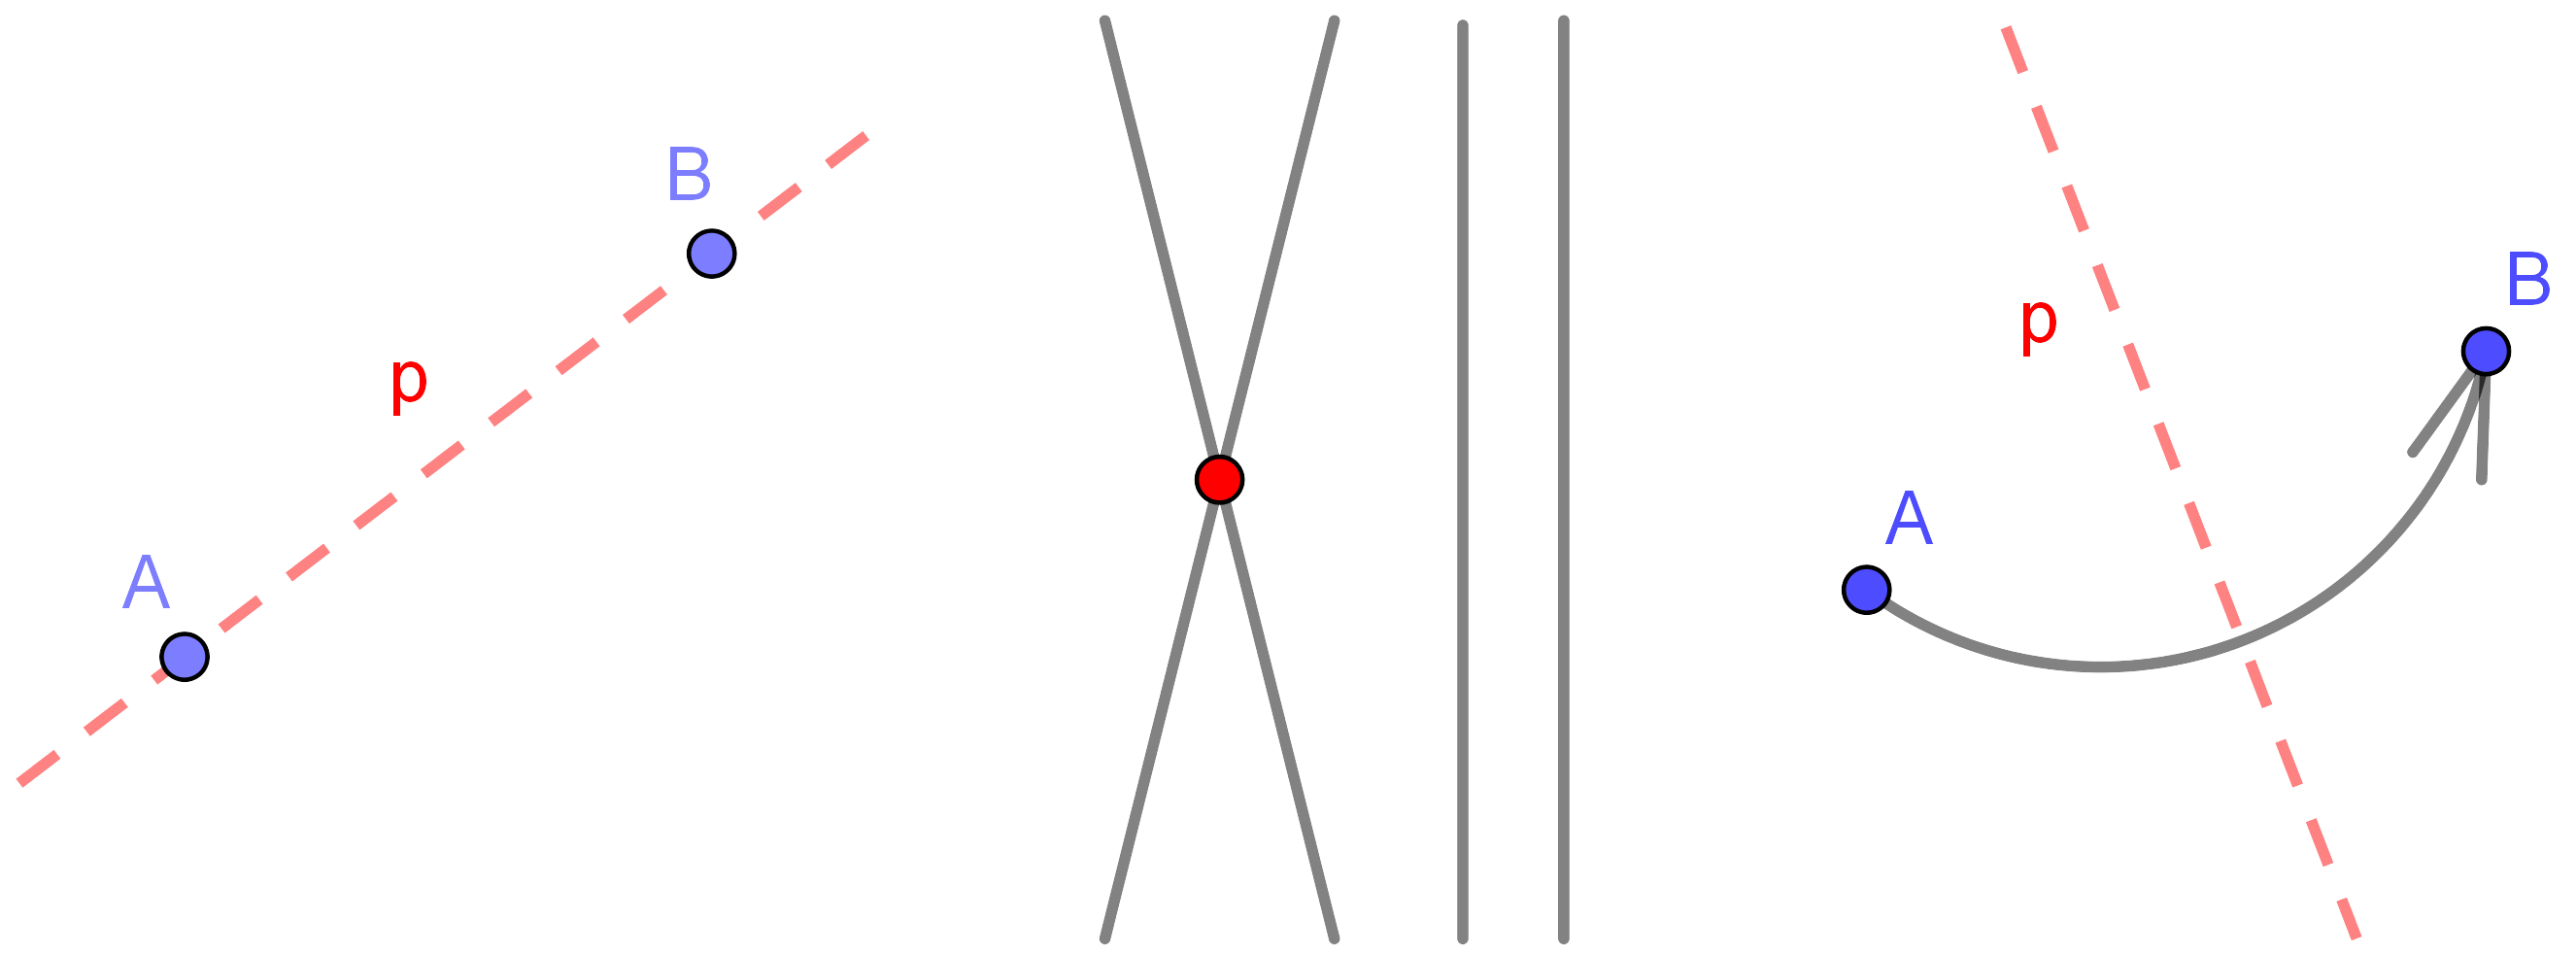
\includegraphics[width=0.6\textwidth]{images/origami_operacije/O1doO3.png}
    \caption[Operacije~\ref{op:O1},~\ref{op:O2} in~\ref{op:O3}]{Operacije (od leve proti desni)~\ref{op:O1},~\ref{op:O2} in~\ref{op:O3}.}
    \label{fig:O1-O3}
\end{figure}

Operacijo~\ref{op:O4} izvedemo tako, da premici položimo drugo na drugo. Očitno mora njuno presečišče (če sta nevzporedni) ležati na pregibu. Opazimo, da nam operacija~\ref{op:O4} konstruira obe simetrali kota, ki ga določata premici in njuno presečišče, v primeru vzporednih premic pa dobimo tretjo vzporednico, ki leži na sredi med njima (slika~\ref{fig:O4}). Zato sta tu možna po dva ali, v posebnem primeru, en pregib.

\begin{figure}[h]
    \centering
    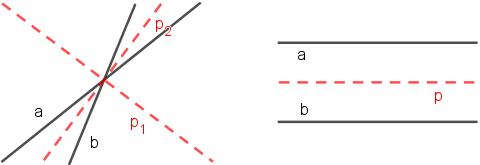
\includegraphics[width=0.5\textwidth]{images/origami_operacije/O4.png}
    \caption[Operacija~\ref{op:O4}]{Operacija~\ref{op:O4} v obeh možnih primerih.}
    \label{fig:O4}
\end{figure}

Operacija~\ref{op:O5} nam podaja konstrukcijo pravokotnice na premico skozi dano točko (slika~\ref{fig:O5}). Pri tem je vseeno, ali točka leži na premici ali ne. Pregib opravimo tako, da premico $a$ položimo samo nase in da hkrati točka $A$ leži na pregibu. Zaradi simetrije je pregib res pravokoten na premico in tako tudi en sam.

\begin{figure}[h]
    \centering
    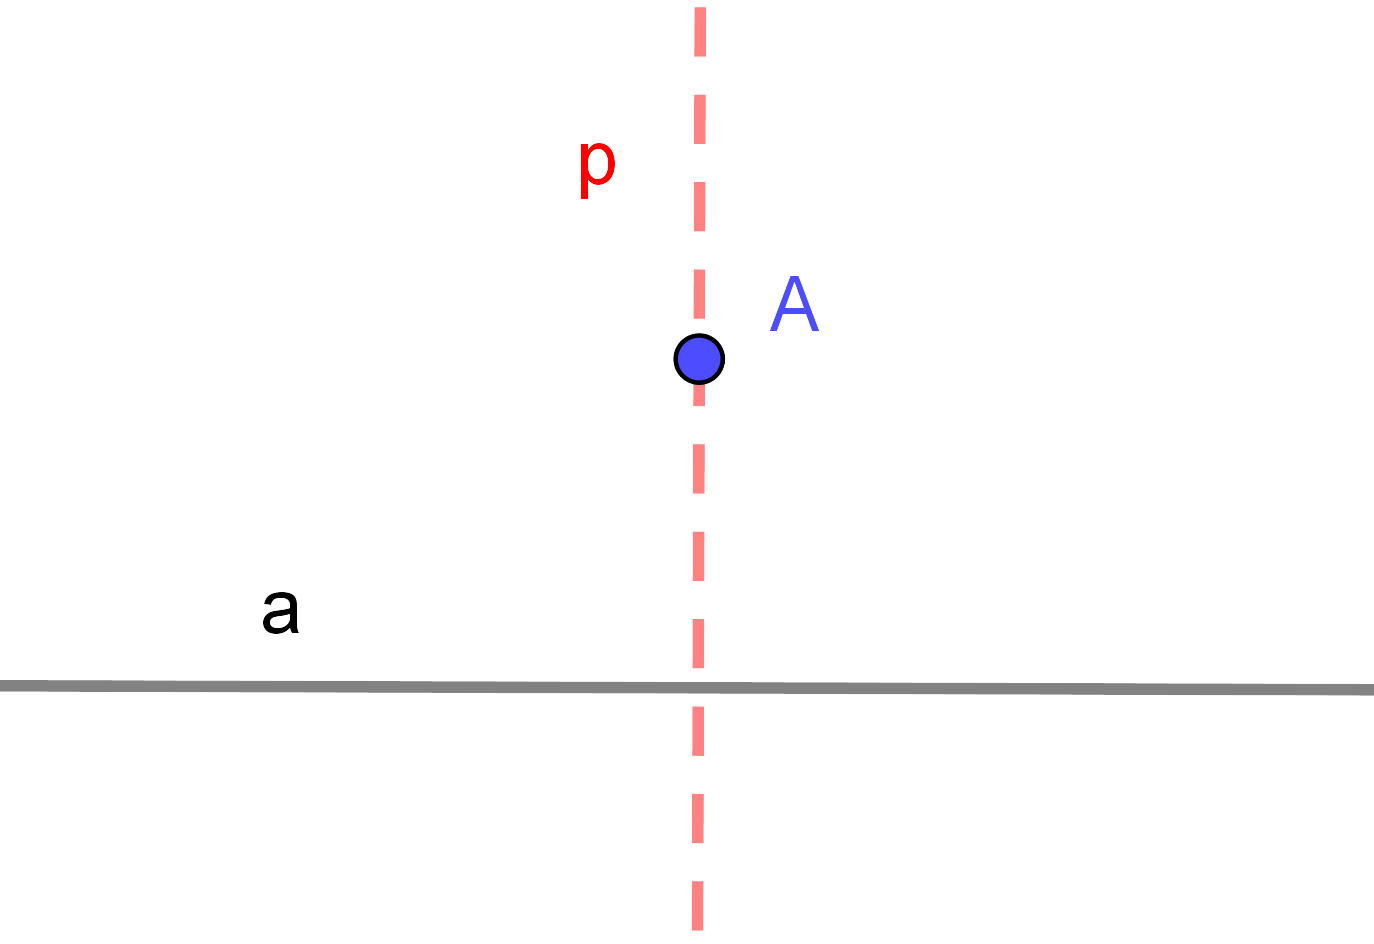
\includegraphics[width=0.3\textwidth]{images/origami_operacije/O5.png}
    \caption[Operacija~\ref{op:O5}]{Operacija~\ref{op:O5}.}
    \label{fig:O5}
\end{figure}

Operacija~\ref{op:O6} je še posebej zanimiva. Pri njeni konstrukciji iščemo pregib skozi točko $B$, ki točko $A$ položi na premico $a$. S prstom upognemo papir čez točko $B$ in tam držimo, nato pa del papirja s točko $A$ premikamo po drugem delu, dokler se točka $A$ ne dotakne premice $a$. Takrat prepognemo po celotni dolžini pregiba.

Poglejmo konstrukcijo še iz evklidskega vidika. Ker točka $B$ leži na pregibu, je enako oddaljena tako od točke $A$ kot tudi njene slike $A'$ na premici $a$, torej je $A'$ ravno presečišče premice $a$ in krožnice s središčem v $B$ ter polmerom $AB$. Pregib je simetrala daljice $AA'$, ki po konstrukciji poteka skozi točko $B$. Če velja $ d(A,B) > d(B,a) $, sta presečišči s premico $a$ dve (in s tem tudi dva možna pregiba, gl.\ sliko~\ref{fig:O6} levo), v primeru $ d(A,B) = d(B,a) $ je presečišče eno samo (in s tem en možen pregib, gl.\ sliko~\ref{fig:O6} na sredi) in je premica $a$ takrat tangentna na omenjeno krožnico, v zadnjem primeru, ko velja $ d(A,B) < d(B,a) $, pa presečišč ni (in s tem tudi pregiba, gl.\ sliko~\ref{fig:O6} desno).

\begin{figure}[h]
    \centering
    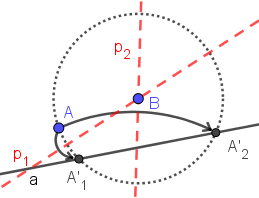
\includegraphics[width=0.3\textwidth]{images/origami_operacije/O6a.png}
    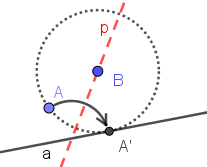
\includegraphics[width=0.25\textwidth]{images/origami_operacije/O6b.png}
    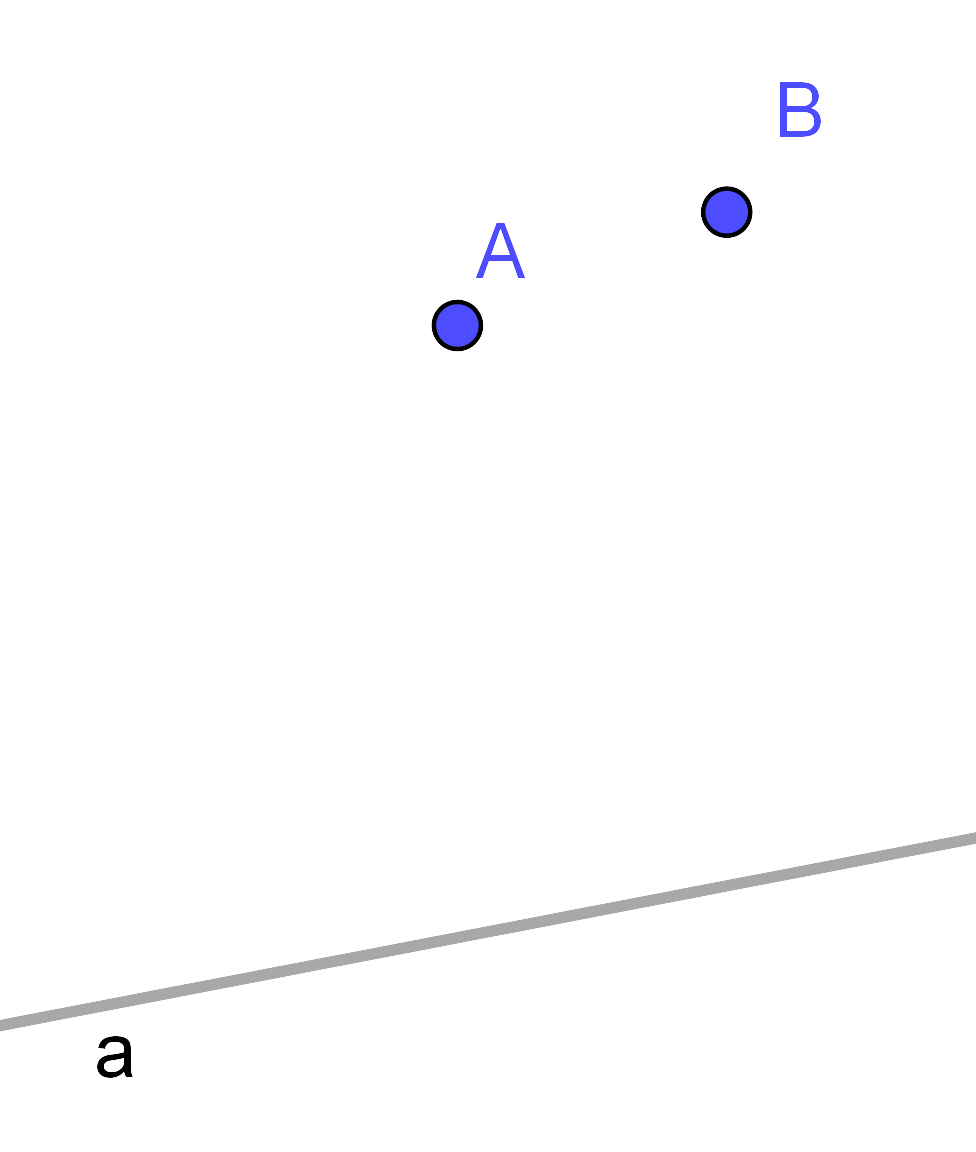
\includegraphics[width=0.2\textwidth]{images/origami_operacije/O6c.png}
    \caption[Operacija~\ref{op:O6}]{Operacija~\ref{op:O6} v vseh treh primerih.}
    \label{fig:O6}
\end{figure}

Zgodba operacije~\ref{op:O6} se tu še ne zaključi. Ker na pregibu ležijo vse točke, ki so enako oddaljene od točke $A$ in $A'$, to velja tudi za točko $P$, ki jo dobimo kot presečišče pregiba in pravokotnice na premico $a$ skozi $A'$ (slika~\ref{fig:O6_parabola}). To je edina točka $P$ na pregibu, za katero velja $ d(A,P) = d(P,a) $ (v srednjem primeru na sliki~\ref{fig:O6} je to kar točka $B$), kar pomeni, da točka $P$ leži na paraboli z goriščem $A$ in premico vodnico $a$. Pregib torej seka parabolo le v eni točki, kar pomeni, da je to \emph{tangenta na to parabolo}. V levem primeru na sliki~\ref{fig:O6} smo dobili dve tangenti.
\footnote{Bolj znanih pod imenom \emph{Huzita-Hatori aksiomi}, vendar izraz \emph{aksiom} tu ni primeren, saj bomo kmalu pokazali, da se med seboj prepletajo in so nekateri izmed njih kombinacija drugih. Prav tako v tej nalogi v ime seznama ne vključimo imen avtorjev, ker je seznam delo veliko več matematikov kot le Hatorija in Huzite.}
\begin{figure}[h]
    \centering
    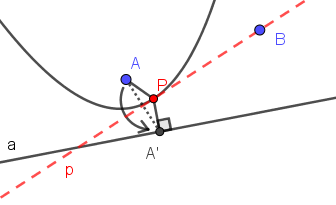
\includegraphics[width=0.4\textwidth]{images/origami_operacije/O6_parabola.png}
    \caption[Tangenta na parabolo]{Konstrukcija tangente na parabolo z goriščem v $A$ in premico vodnico $a$.}
    \label{fig:O6_parabola}
\end{figure}

Poglejmo si naslednjo operacijo. Konstrukcijo~\ref{op:O7} začnemo z upogibom papirja, ki točko $A$ položi na premico $a$, potem pa en upognjen del papirja po drugem delu premaknemo tako, da točka $A$ ostane na premici $a$ (med premikanjem papirja se lahko premika po premici) in se točka $B$ stakne s premico $b$. Takrat naredimo pregib. Na sliki~\ref{fig:O7} so za isto izbiro točk in premic prikazani trije pregibi, kar je tudi največje možno število pregibov za iste točke in premice. Več o številu pregibov pri tej operaciji je pojasnjenega v začetku poglavja~\ref{pogl:enacbe}.

\begin{figure}[h]
    \centering
    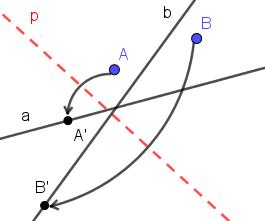
\includegraphics[width=0.3\textwidth]{images/origami_operacije/O7b.png}
    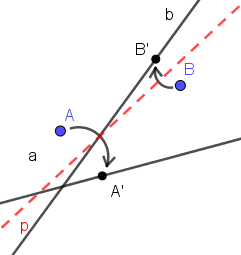
\includegraphics[width=0.25\textwidth]{images/origami_operacije/O7a.png}
    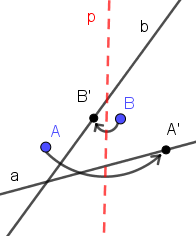
\includegraphics[width=0.2\textwidth]{images/origami_operacije/O7c.png}
    \caption[Operacija~\ref{op:O7}]{Operacija~\ref{op:O7} (primer treh pregibov za isti točki in premici).}
    \label{fig:O7}
\end{figure}

Kaj je geometrijski pomen te operacije? Če smo pri operaciji~\ref{op:O6} dobili tangento na parabolo, potem lahko takoj vidimo, da pri operaciji~\ref{op:O7} dobimo \emph{skupno tangento na dve paraboli} -- ena ima gorišče v točki $A$ in premico vodnico $a$, druga pa gorišče v točki $B$ ter premico vodnico $b$ (slika~\ref{fig:O7_paraboli}).

\begin{figure}[h]
    \centering
    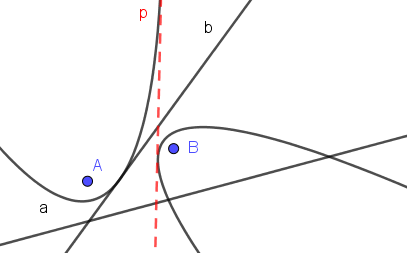
\includegraphics[width=0.5\textwidth]{images/origami_operacije/O7c_paraboli.png}
    \caption[Skupna tangenta na dve paraboli]{Operacija~\ref{op:O7} kot konstrukcija skupne tangente na dve paraboli.}
    \label{fig:O7_paraboli}
\end{figure}

\begin{opomba}
    O pregibu iz operacije~\ref{op:O7} naj bi prva pisala italijanski matematičarki Margherita P.\ Beloch, po kateri operacijo imenujemo tudi \emph{Belochin pregib}.
\end{opomba}

Zadnja operacija~\ref{op:O8} zahteva nevzporedni premici, saj v nasprotnem primeru ne moremo konstruirati pregiba, ki bi bil pravokoten na obe premici in točko $A$ položil na premico $a$ (razen če le-ta že leži na njej). Konstrukcijo začnemo tako, da opravimo rahel upogib, pravokoten na premico $b$. Upogib premikamo po tej premici (še vedno ohranjamo njegovo pravokotnost nanjo), dokler se točka $A$ ne dotakne premice $a$.

Premislimo še njegovo evklidsko konstrukcijo: ker mora biti pregib pravokoten na premico $b$, bo slika točke $A$ (označena z $A'$) ležala na vzporednici skozi točko $A$ k premici $b$. Prav tako mora točka $A'$ ležati na premici $a$, torej je slika ravno presečišče omenjene vzporednice in premice $a$. Iskan pregib je simetrala daljice $AA'$, ki je po konstrukciji pravokoten na premico $b$ (slika~\ref{fig:O8}).

\begin{figure}[h]
    \centering
    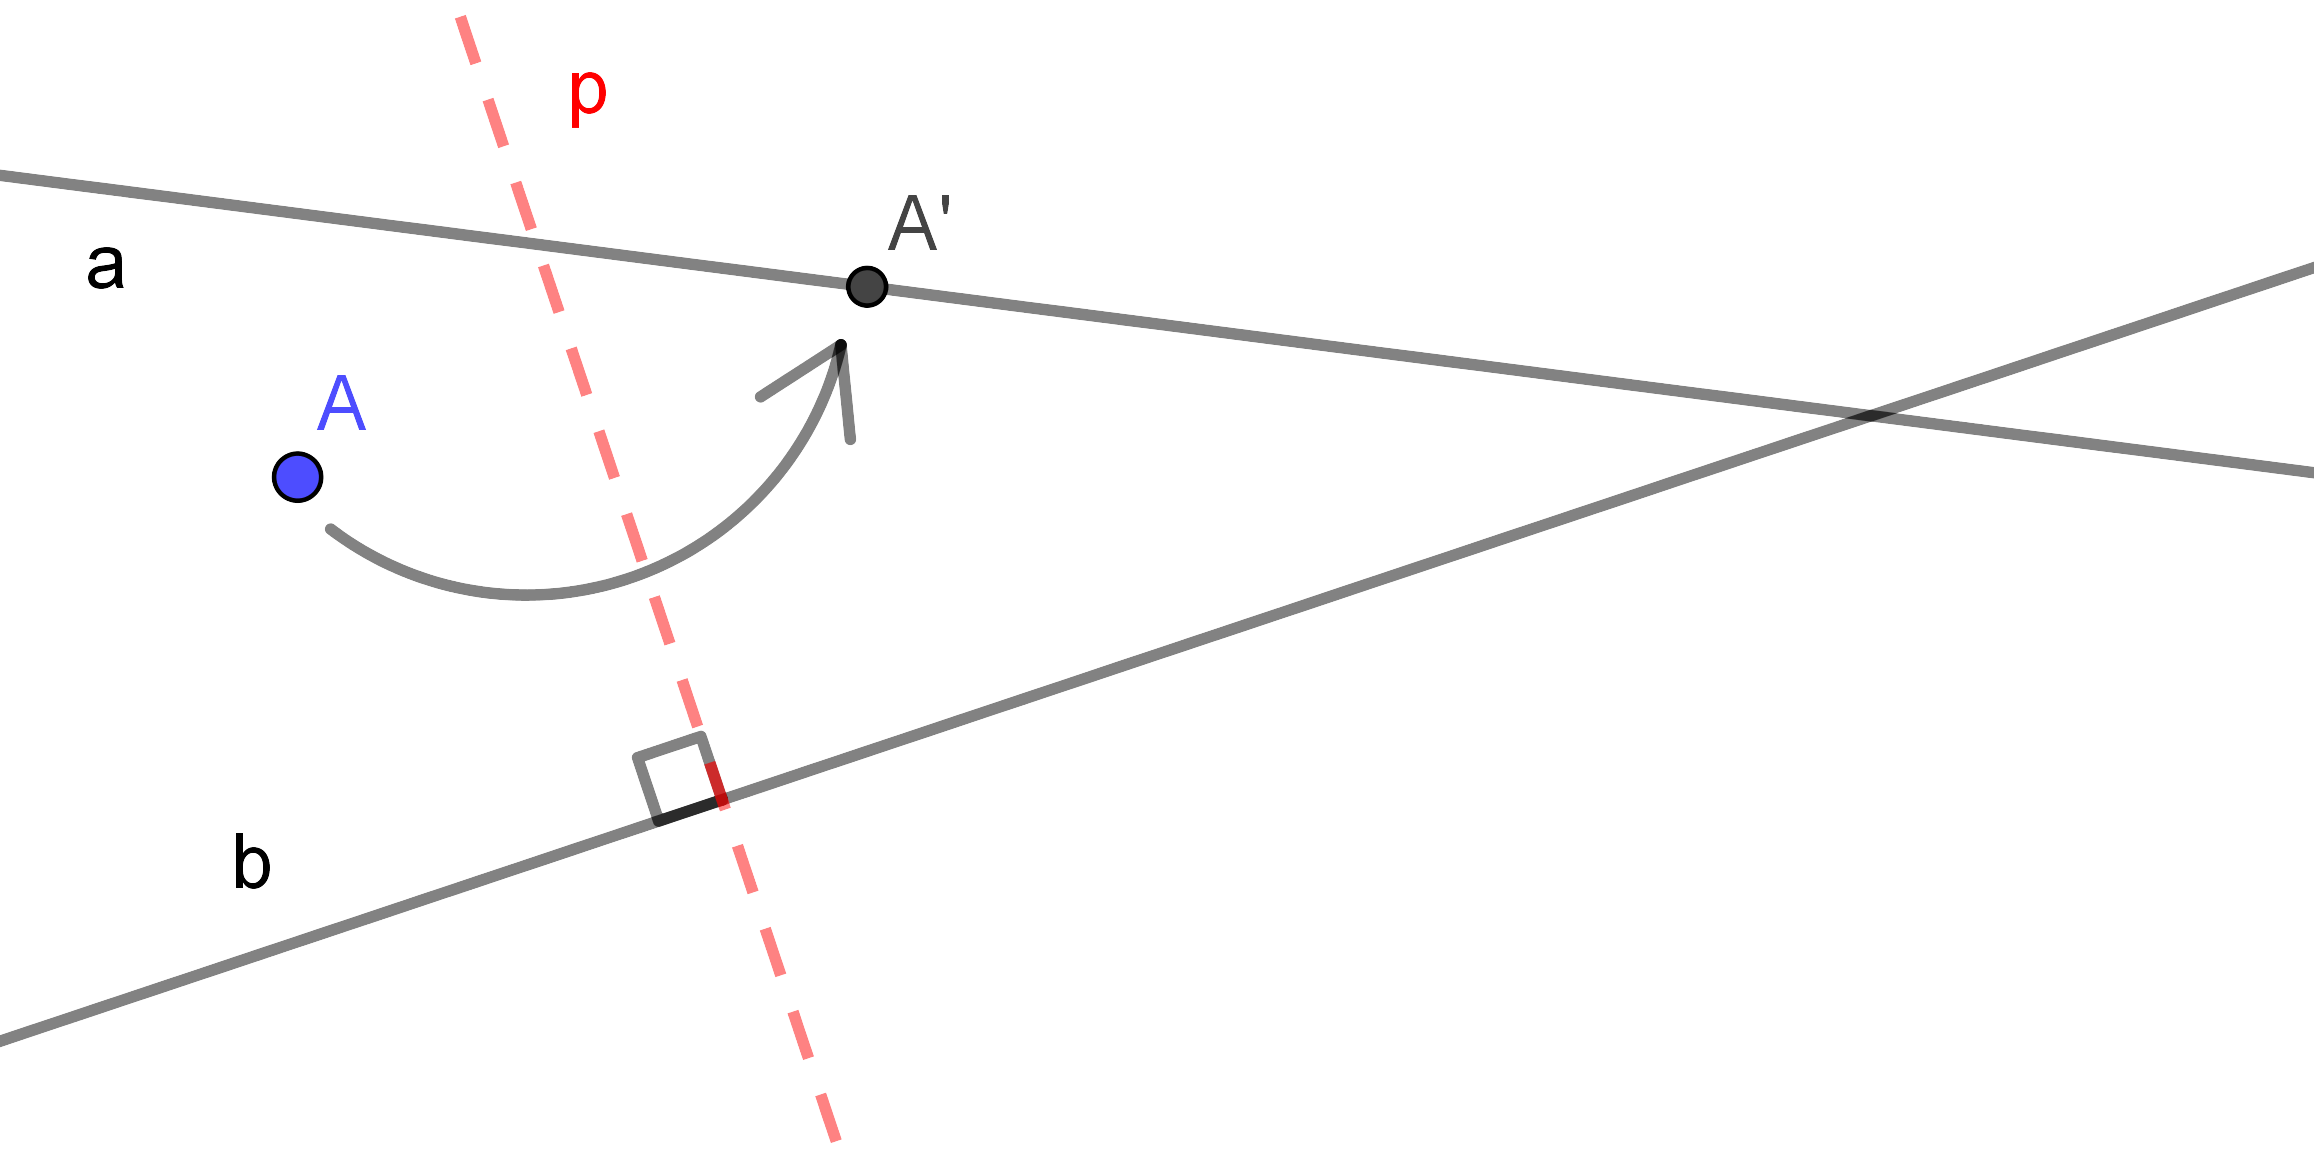
\includegraphics[width=0.6\textwidth]{images/origami_operacije/O8.png}
    \caption[Operacija~\ref{op:O8}]{Operacija~\ref{op:O8}.}
    \label{fig:O8}
\end{figure}

\opomba{Origami operacije ne podajajo konstrukcije slik točk, temveč samo pregibe, ki točke preslikajo na premice. Sliko točke konstruiramo šele po uporabi operacije~\ref{op:O5} -- skozi originalno točko naredimo pregib, pravokoten na pregib iz izbrane operacije, in slika je presečišče te pravokotnice in premice, na katero smo prepognili originalno točko.}

\subsubsection*{Zadostne in potrebne origami operacije}
\label{podpogl:zadost_potr_op}

Omenili smo že, da je teh osem operacij zadostnih za katerokoli origami konstrukcijo, kar nam pove naslednji izrek. Njegov dokaz izpustimo (bralec si ga skupaj s slikovno ponazoritvijo lahko pogleda v~\cite[str.\ 24--26 (izrek 1.1)]{hull2020}), njegova ideja pa je, da vsak možen prepogib, ki prekrije točko ali premico s točko ali premico (gl.\ seznam petih možnosti v začetku razdelka~\ref{origami_konstrukcije}) uvrstimo v eno izmed origami operacij~\ref{op:O1}--\ref{op:O8}.

\begin{izrek}
    \label{izr:op1do8}
    Če dovolimo le enkratne in ravne pregibe, so edine možne operacije prepogibanja operacije~\ref{op:O1}--\ref{op:O8}.
\end{izrek}

Vendar ali so vse te operacije tudi potrebne -- lahko katero izpustimo? Operacija~\ref{op:O2} je očitno potrebna, saj nam edina določa nove točke. Če podrobneje opazujemo ostale konstrukcije, pa opazimo, da so vse posebni primeri operacije~\ref{op:O7}, ko premici $a$ in $b$ sovpadata ali ko ena ali obe izmed točk $A$ in $B$ ležita na premici:
\begin{itemize}
    \item Operacija~\ref{op:O1}: Naj točka $A$ leži na premici $a$, točka $B$ pa na premici $b$. Pregib skozi točki $A$ in $B$ točko $A$ ohrani na premici $a$ in točko $B$ na premici $b$.
    \item Operacija~\ref{op:O3}: Naj točka $A$ leži na premici $b$, točka $B$ pa na premici $a$. Pregib, ki položi točki drugo na drugo, točko $A$ položi na premico $a$ in hkrati točko $B$ na premico $b$ .
    \item Operacija~\ref{op:O4}: Naj točka $A$ leži na premici $b$, točka $B$ pa na premici $a$. Simetrala kota v presečišču premic (ali vmesna vzporednica, če sta premici $a$ in $b$ vzporedni), točko $A$ položi na premico $a$ in hkrati točko $B$ na premico $b$.
    \item Operacija~\ref{op:O5}: Naj točka $A$ leži na premici $a$, točka $B$ pa na premici $b$. Pregib skozi točko $A$ (ali $B$), ki je pravokoten na premico $b$ (ali $a$), točko $A$ ohrani na premici $a$ in točko $B$ na premici $b$.
    \item Operacija~\ref{op:O6}: Naj točka $B$ leži na premici $b$. Pregib skozi točko $B$, ki točko $A$ preslika na premico $a$ (če tak pregib obstaja), točko $B$ ohrani na premici $b$.
    \item Operacija~\ref{op:O8}: Naj točka $B$ leži na premici $b$. Pregib, ki točko $A$ položi na premico $a$ in je pravokoten na premico $b$, točko $B$ ohrani na premici $b$.
\end{itemize}

Ker lahko vse konstrukcije po izreku~\ref{izr:op1do8} opišemo z operacijami~\ref{op:O1}--\ref{op:O8}, smo s tem dokazali spodnji izrek:

\begin{izrek}
    \label{izr:dve_operaciji}
    Če imamo dani vsaj dve točki in dve nevzporedni premici, ki vsebujeta dane točke, potem lahko vse origami konstrukcije z enkratnimi in ravnimi pregibi opišemo s kombinacijo operacij~\ref{op:O2} in~\ref{op:O7}.
\end{izrek}
\begin{opomba}
    V izreku lahko namesto dveh nevzporednih premic vzamemo le eno premico, ki vsebuje obe točki. Operacija~\ref{op:O4} v tem primeru ni izvedljiva, saj za simetralo kota potrebujemo dve premici, sicer pa vsi pregibi iz operacij~\ref{op:O1}--\ref{op:O8} (razen~\ref{op:O4}) potekajo ali po tej premici ali pa so pravokotni nanjo v eni izmed točk. 
\end{opomba}

Kljub temu bomo pri opisu origami konstrukcij uporabljali vseh osem aksiom operacij, saj bomo kakšen pregib lažje razložili preko ene od ostalih petih operacij kot pa opisovali, na kakšen način je to operacija~\ref{op:O7}.

\subsubsection{Zrcaljenje točke čez premico}
\label{podpogl:zrcaljenje_origami}

Operacija~\ref{op:O3} nam poda simetralo daljice $AB$. Torej je točka $B$ zrcalna slika točke $A$ čez to premico. Kaj pa, če imamo za neko točko $A$ že dano premico $a$ in iščemo njeno zrcalno sliko?

Naravna rešitev je, da naredimo pregib po premici in s svinčnikom označimo zrcalno sliko. A ker po definiciji~\ref{def:origami_konstruktibilnost}, ki pravi, da lahko točke dobimo le kot presečišča pregibov, in ker je uporaba pisala dovoljena le za vidnejšo označbo že konstruiranih točk, tega ne smemo storiti. Zato moramo najti zaporedje pregibov, kjer na koncu kot presečišče nekih dveh premic dobimo želeno točko.

Za dano premico $a$ in točko $A$, ki ne leži na tej premici (sicer je točka $A$ zrcalna slika sama sebi), lahko zrcalno sliko točke konstruiramo z naslednjimi koraki (prikazani na sliki~\ref{fig:zrcaljenje_cez_premico}, postopek vzet iz~\cite[str.\ 28]{hull2020}):
\begin{enumerate}
    \item Z operacijo~\ref{op:O5} prepognemo pravokotnico na premico $a$ skozi točko $A$.
    \item Z operacijo~\ref{op:O4} prepognemo simetralo kota, ki ga oklepata premica $a$ in pravokotnica iz prvega koraka.
    \item Z operacijo~\ref{op:O5} prepognemo pravokotnico na simetralo skozi točko $A$. Njeno presečišče s premico $a$ označimo z $B$.
    \item Z operacijo~\ref{op:O5} prepognemo pravokotnico na pregib iz tretjega koraka skozi točko $B$. Presečišče novega pregiba in pravokotnice iz prvega koraka označimo z $A'$.
\end{enumerate}

\begin{figure}[h]
    \centering
    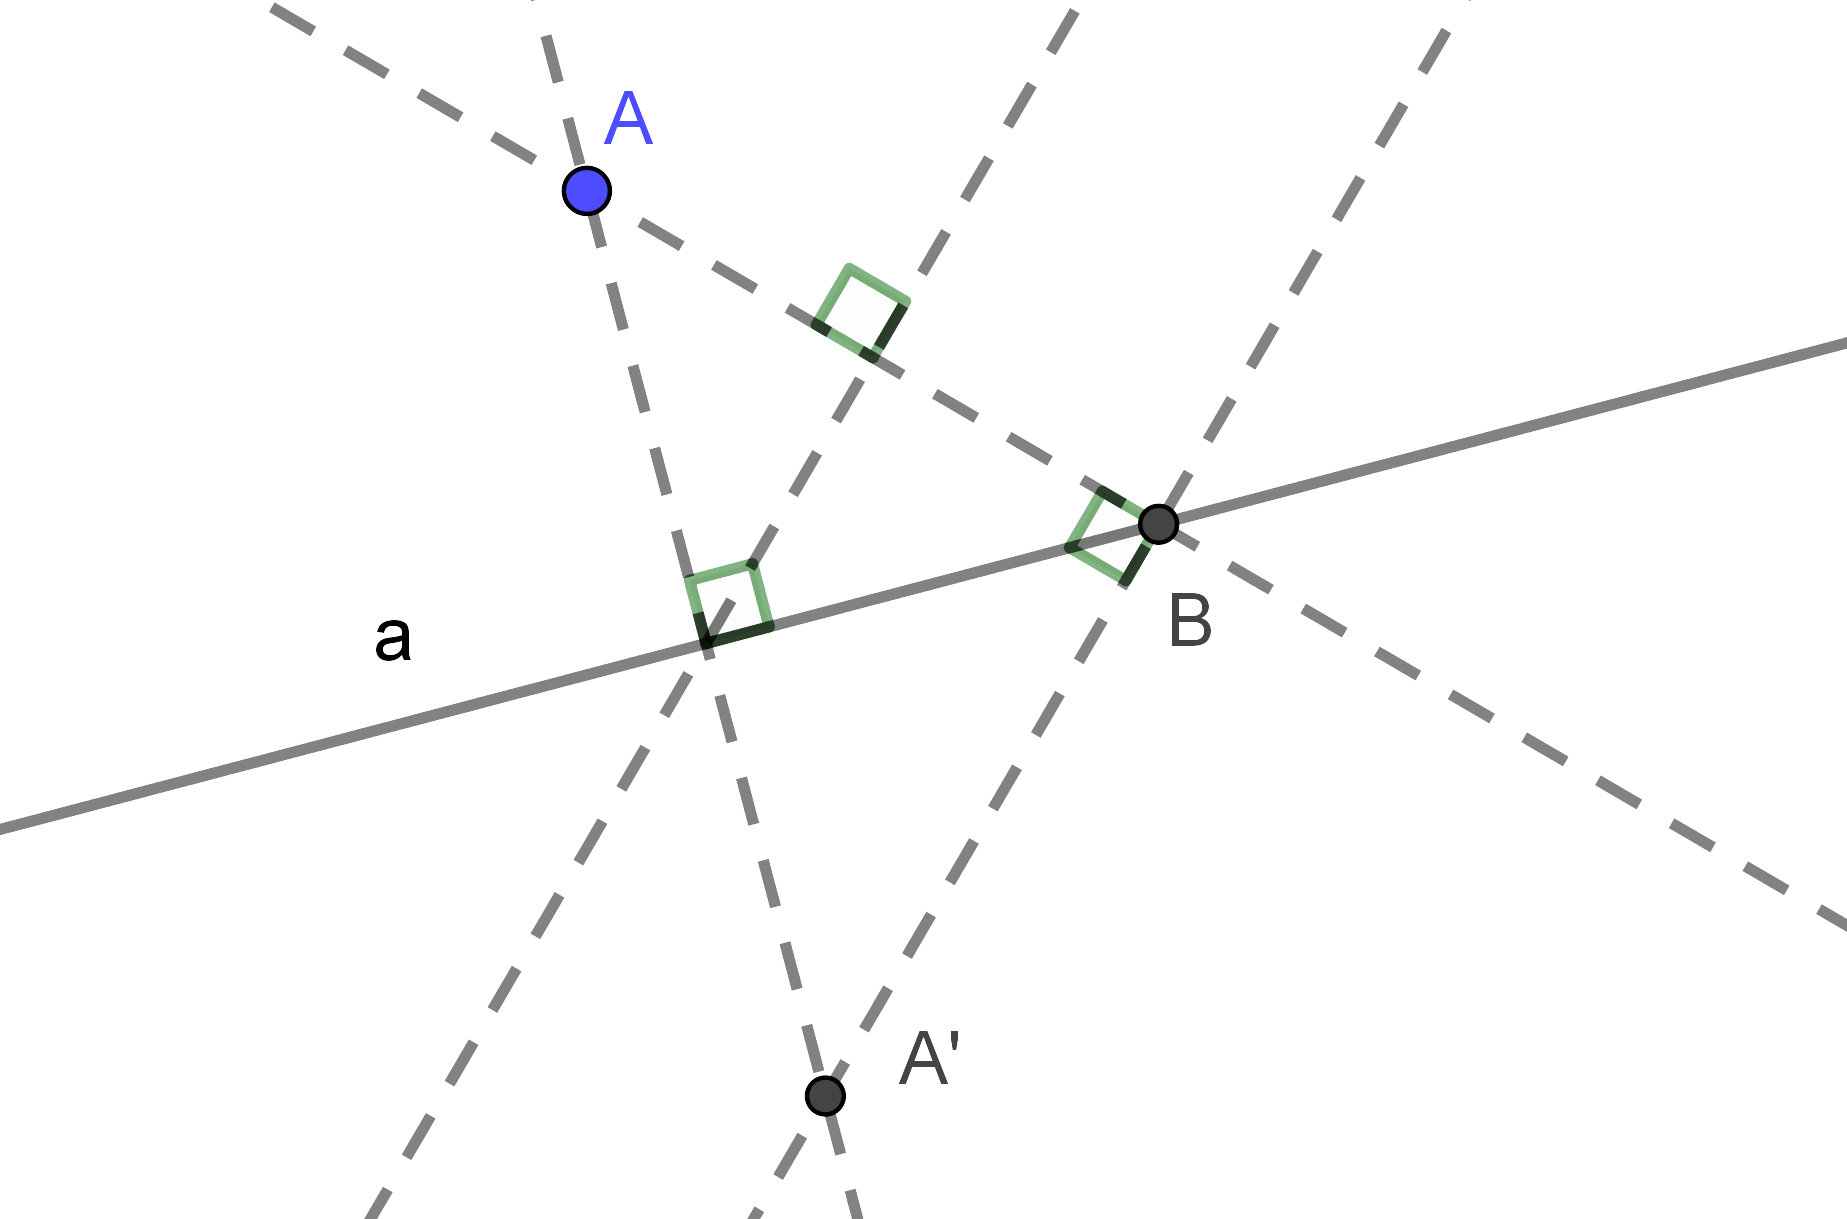
\includegraphics[width=0.4\textwidth]{images/zrcaljenje_tocke_cez_premico.png}
    \caption[Zrcaljenje čez premico]{Zrcaljenje točke $A$ čez premico $a$ s prepogibanjem papirja.}
    \label{fig:zrcaljenje_cez_premico}
\end{figure}

\begin{trditev}
    Točka $A'$ iz opisane konstrukcije je zrcalna slika točke $A$.
\end{trditev}

\begin{dokaz}
    Trikotnik, ki ga dobimo po 3.\ koraku, je pravokoten in enakokrak, saj je simetrala (pravega kota) iz 2.\ koraka pravokotna na njegovo osnovnico. Zato kot ob točki $A$ znaša $45^{\circ}$. Ker je trikotnik $\triangle A'BA$ pravokoten, je zato tudi enakokrak, torej premica $a$ razpolavlja daljico $AA'$, torej je $A'$ res zrcalna slika točke $A$.
\end{dokaz}

Ker lahko čez premico zrcalimo točke, lahko čeznjo zrcalimo tudi daljice oz.\ premice -- to storimo tako, da zrcalimo dve točki z daljice in naredimo pregib čez njuni sliki.

% Moja avtorska trditev in dokaz:)

\begin{trditev}
    \label{trd:prenasanje_razdalj}
    Z ravnimi in enkratnimi prepogibi ter upoštevanjem origami operacij lahko s prepogibanjem papirja prenašamo razdalje.
\end{trditev}

\begin{dokaz}
    V ravnini si izberimo poljubni točki $A$ in $B$, ki določata daljico z neko dolžino $r$. Naj bo $a$ poljubna premica in $A'$ poljubna točka na njej. Trditev pravi, da lahko z origami operacijami konstruiramo točko $B' \in a$, da je $d(A', B') =r$ (slika~\ref{fig:prenos_razdalje_konec}). Pri tem ni pomembno, na kateri strani točke $A'$ leži točka $B'$, saj jo lahko vedno zrcalimo čeznjo.

    \begin{figure}[h]
        \centering
        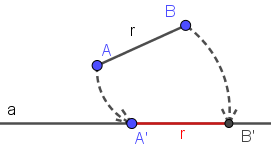
\includegraphics[width=0.35\textwidth]{images/zrcaljenje_konec.png}
        \caption[Prenašanje razdalj z origamijem]{Prenos dolžine daljice $AB$ na premico $a$ k izbrani točki $A'$.}
        \label{fig:prenos_razdalje_konec}
    \end{figure}
    
    Prenos razdalje razdelimo na dva koraka:
    \begin{enumerate}
        \item Če $A \neq A'$, daljico $AB$ zrcalimo čez tisto premico $p$, ki točko $A$ preslika v točko $A'$ (po~\ref{op:O3} je tak pregib oz.\ premica ena sama). Zrcalno sliko točke $B$ označimo z $B''$ (slika~\ref{fig:prenos_razdalje_koraki} levo). V posebnem primeru, ko daljica $AB$ leži na premici $a$, je to že konec konstrukcije. 
        \item Daljico $A'B''$ zavrtimo okoli krajišča $A'$, da se točka $B''$ preslika na premico $a$. To storimo tako, da z operacijo~\ref{op:O4} konstruiramo simetralo kota med daljico $A'B''$ in premico $a$ in čeznjo zrcalimo točko $B''$ (slika~\ref{fig:prenos_razdalje_koraki} desno). S tem dobimo točko $B' \in a$, ki je po konstrukciji od točke $A'$ oddaljena za dolžino $r$.
    \end{enumerate}
    S tem smo razdaljo $r$ prenesli na poljubno mesto v ravnini.

    \begin{figure}[h]
        \centering
        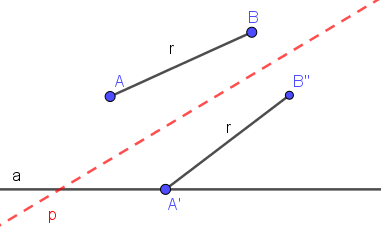
\includegraphics[width=0.45\textwidth]{images/zrcaljenje_korak1.png}
        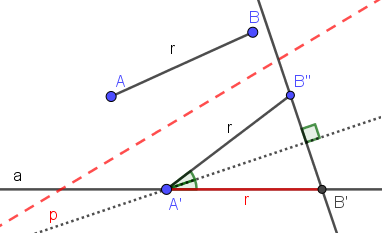
\includegraphics[width=0.45\textwidth]{images/zrcaljenje_korak2.png}
        \caption[Prenašanje razdalj z origamijem po korakih]{Zrcaljenje daljice $AB$ (levo) in rotacija daljice čez eno krajišče (desno).}
        \label{fig:prenos_razdalje_koraki}
    \end{figure}
\end{dokaz}

Tako lahko s prepogibanjem papirja zrcalimo točke (in premice), prenašamo razdalje pa tudi -- po 2.\ koraku iz zgornjega dokaza -- rotiramo točke (in premice). Od sedaj naprej pa bomo pri konstrukcijah, ki vključujejo zrcaljenje točk ali premic, zaradi preglednosti izpustili potrebne pregibe in zrcaljene točke konstruirali kar z ravnilom in označili s svinčnikom.

\subsection{Zakaj origami konstrukcije nadvladajo evklidske}
\label{podpogl:nadvlada_origamija}

Prišli smo do ključnega dela poglavja -- reševanje vprašanja, zakaj se nam z origami konstrukcijami sploh splača ukvarjati.

Tako z evklidskim orodjem kot s prepogibanjem papirja lahko konstruiramo premice in točke ter prenašamo razdalje. Le evklidskim orodjem lahko konstruiramo tudi krožne loke, ker pa znamo rotirati točke okoli druge točke, lahko tudi s prepogibanjem papirja konstruiramo katerokoli točko na krožnici z danim središčem in polmerom. Tako lahko vse evklidske konstrukcije opravimo tudi z origamijem (za natančnejši dokaz glej~\cite[str.\ 362--365]{geret1995}).

Ob posameznih opisih operacij~\ref{op:O1}, \ref{op:O3}, \ref{op:O4}, \ref{op:O5}, \ref{op:O6} in \ref{op:O8} smo že premislili, kako  jih je mogoče opraviti tudi z evklidskim orodjem. Tudi operacija~\ref{op:O2} je od evklidskih konstrukcij že znana. Do tu nam torej origami konstrukcije niso dale ničesar novega.

Ključna je sedma operacija. Izkaže se namreč, da operacije~\ref{op:O7} oz.\ Belochinega pregiba ne moremo opraviti z evklidskim orodjem. Kako lahko to dokažemo? V poglavju~\ref{pogl:starogrskiproblemi} bomo med drugim spoznali več origami postopkov, ki nam poljuben kot razdelijo na tri skladne dele, pri tem pa uporabimo pregib iz operacije~\ref{op:O7}. Ker \emph{trisekcija kota z evklidskim orodjem ni mogoča} (gl.\ konec razdelka~\ref{podpogl:evkl_konstruktibilnost}), posledično tudi konstrukcija operacije~\ref{op:O7} s tem orodjem ne obstaja. Prav tako bomo v poglavju~\ref{pogl:enacbe} videli več načinov uporabe operacije~\ref{op:O7} za reševanje kubične enačbe, za katero prav tako vemo, da je v splošnem z evklidskim orodjem ne moremo rešiti.

Sedaj vemo, da je množica evklidskih konstrukcij \emph{prava} podmnožica origami konstrukcij. V naslednjem razdelku si bomo pogledali, kako lahko evklidske in origami konstrukcije prevedemo v jezik algebre in tudi na algebrski način pokažemo premoč origamija nad evklidskim orodjem. Raziskovali bomo, katere dolžine (in s tem katera števila) lahko z obema orodjema konstruiramo. Tak pogled je imel že Evklid, ki je na števila gledal kot končni rezultat niza konstrukcij z evklidskim orodjem pri dani daljici enotske dolžine~\cite[str. 164]{michael2005}.

\subsubsection{Algebrski pogled na evklidske konstrukcije}
\label{podpogl:evkl_konstruktibilnost}

\begin{definicija}
    \label{def:evkl_konstr}
    Na listu papirja, ki nam služi kot model ravnine $\C$, imejmo dano izhodišče $O$ in število $1$ na realni osi. Če lahko z neoznačenim ravnilom in šestilom s končnim številom potez konstruiramo kompleksno število $\alpha$, rečemo, da je $\alpha$ \emph{evklidsko-konstruktibilno} število.
\end{definicija}

Kompleksna ravnina $\C$ je v bijekciji z ravnino $\R^2$. Če lahko z evklidskim orodjem konstruiramo število $\alpha = a + bi$, lahko torej konstruiramo točko $(a, b)$ in obratno. Tako je dovolj obravnavati evklidske konstrukcije v realni ravnini.

Iz definicije~\ref{def:evklidske_konstrukcije} evklidskih konstrukcij se spomnimo, da lahko premico konstruiramo le skozi poljubni dve dani točki, krožnico s središčem v poljubni dani točki in poljubno dano točko na njej, točke z evklidskim orodjem pa dobimo le kot presečišče dveh premic, dveh krožnic ali premice in krožnice.

\begin{definicija}
    Točki, ki jo lahko v ravnini $\R^2$ konstruiramo z evklidskim orodjem, pravimo \emph{evklidsko-konstruktibilna točka}. Enako definiramo \emph{evklidsko-konstruktibilno premico} in \emph{evklidsko-konstruktibilno krožnico}.
\end{definicija}

Radi bi določili množico vseh evklidsko-konstruktibilnih števil. Torej iščemo, katere vse možne točke v ravnini $\R^2$ lahko konstruiramo z evklidskim orodjem. Naslednja lema nam iskanje še poenostavi.

\begin{lema}
    \label{trd:bijekcija_CR}
    Naj bo $\alpha = a+bi \in \C$, kjer $a, b \in \R$. Potem je $\alpha$ evklidsko-konstruktibilno število, če in samo če sta $a, b$ evklidsko-konstruktibilni števili.
\end{lema}
\begin{dokaz}
    Ker sta $a$ in $b$ pravokotni projekciji števila $\alpha$ na realno in imaginarno os -- bralec naj premisli, kako ju lahko konstruiramo z evklidskim orodjem --, je trditev očitna.
\end{dokaz}

Iščemo, katere realne koordinate so evklidsko-konstruktibilne, torej v resnici iščemo množico \emph{realnih} evklidsko-konstruktibilnih števil. Označimo jo z $\E$. Po definiciji~\ref{def:evkl_konstr} velja $0, 1 \in \E$, po lemi~\ref{trd:bijekcija_CR} pa $\alpha = a + bi$ je evklidsko-konstruktibilno število natanko takrat, ko velja $a, b \in \E$.

\begin{trditev}
    Naj bodo $a, b, c \in \E, c \neq 0$. Potem so tudi števila $a+b, \; a-b, \; ab, \; a/c$ in $\sqrt{a}$ elementi množice $\E$.
\end{trditev}

Dokaz tu opustimo. Bralec si ga lahko ogleda v~\cite{jerman1998}, \cite[str.\ 165--170]{michael2005} ali pa v dokazovanju podobnega izreka za števila, konstruktibilna z origamijem (gl.\ izrek~\ref{izr:podpolje} v nadaljevanju). Iz trditve sledi, da je množica $\E$, ki je podmnožica polja realnih števil, tudi sama polje.

\begin{posledica}
    Množica $\E$ je podpolje polja $\R$.
\end{posledica}

Velja še več -- to, da iz $a \in \E$ sledi $\sqrt{a} \in \E$, je lastnost \emph{evklidskih polj}. Primer evklidskega polja je množica realnih števil, medtem ko npr.\ množica racionalnih števil te lastnosti nima -- za $2 \in \Q$ velja $\sqrt{2} \notin \Q$.

Še vedno pa moramo določiti realna števila, ki sestavljajo množico $\E$. Očitno je, da iz danih števil $0$ in $1$ s seštevanjem in odštevanjem dobimo vsa cela števila, z deljenjem vsa racionalna števila, s korenjenjem pa še njihove kvadratne korene. Naslednja lema je zato očitna.

\begin{lema}
    Naj bo $a \in \Q$. Potem velja $a, \sqrt{a} \in \E$.
\end{lema}

\begin{posledica}
    \label{posl:podmnozice}
    Velja $\Q \subset \E \subset \R$.
\end{posledica}
\begin{dokaz}
    Očitno je množica racionalnih števil prava podmnožica množice $\E$. Ovreči moramo samo možnost $\E = \R$. Vsako število iz množice $\E$ je rezultat seštevanja, odštevanja, množenja, deljenja in korenjenja elementov iz te množice (z začetnima številoma $0$ in $1$), zato je algebraično nad $\Q$ -- je rešitev neke enačbe z racionalnimi koeficienti. Torej v množici $\E$ ne morejo biti transcedentna število, kot je na primer število $\pi$. Zato je $\E$ res prava podmnožica množice $\R$.
\end{dokaz}

Ker je polje $\Q$ podpolje polja $\E$, je $\E$ \emph{razširitev} polja $\Q$. Ideja je, da poiščemo najmanjšo razširitev polja racionalnih števil, ki je zaprta za operacijo kvadratnega korenjenja. To bo naša množica $\E$. V pomoč nam je naslednja trditev.

\begin{trditev}
    \label{trd:kv_razs_prva}
    Naj bo $r \in \Q^+, \sqrt{r} \notin \Q$. Potem je množica $ \Q(\sqrt{r}) = \{ a + b \sqrt{r}; a, b \in \Q \}$ razširitev polja $\Q$.
\end{trditev}
\begin{dokaz}
    Naj bo $r$ poljubno racionalno število po predpostavki trditve. Očitno velja $\Q \subset \Q(\sqrt{r})$, saj so v $\Q(\sqrt{r})$ med drugim tudi vsa števila oblike $a + 0 \cdot \sqrt{r} = a$, kjer je $a \in \Q$ poljubno. Dokazati moramo, da je $\Q(\sqrt{r})$ polje.

    Očitno je $0, 1 \in \Q(\sqrt{r})$, če vzamemo $a \in \{0, 1\}$ in $b = 0$. Bralcu prepustimo lahek računski preostanek dokaza, kjer mora pokazati, da so vsota, razlika, produkt in količnih števil $a_1 + b_1\sqrt{r}$ in $a_2 + b_2\sqrt{r}$ oblike $a_3 + b_3\sqrt{r}$.
\end{dokaz}

Za ustrezen $r$ lahko na enak način poiščemo razširitev polja $\Q(\sqrt{r})$. Vzamemo $q \in \Q(\sqrt{r})^+, \sqrt{q} \notin \Q(\sqrt{r})$. Potem so elementi nove razširitve pola $\Q(\sqrt{r})$ oblike $(a_1 + b_1\sqrt{r}) + (a_2 + b_2\sqrt{r})\sqrt{q}$. Pri tem velja $a_1 + b_1\sqrt{r}, \; a_2 + b_2\sqrt{r} \in \Q(\sqrt{r})$ in $a_1, b_1, a_2, b_2 \in \Q$.

Primer (vzeto iz~\cite[str.\ 36]{geometricconstructions}): Naj bo $F = \Q(\sqrt{5})$, torej so njegovi elemeni oblike $a + b\sqrt{5}$, kjer sta $a, b \in \Q$. Za število $q = (35-15\sqrt{5})/2 \in F^+$ je njegov koren enak številu $\sqrt{q} = (5-3\sqrt{5})/2 \in F$, zato $F(\sqrt{q}) = F$ ni razširitev polja $F$. Za število $2 \in F^+$ pa ne obstajata $a, b \in \Q$, da bi veljalo $\sqrt{2} = a+b\sqrt{5}$, torej $\sqrt{2} \notin F$ in je $F(\sqrt{2})$ razširitev polja $F$. Pišemo $F(\sqrt{2}) = \Q(\sqrt{5}, \sqrt{2})$. 

\begin{definicija}
    \label{def:kvad_razs}
    Naj bo $F_0$ polje in $r \in F_0^+, \sqrt{r} \notin F_0$. Potem polje
    $$ F_0(\sqrt{r}) = \{a+b\sqrt{r}; a,b \in F_0\} $$
    imenujemo \emph{kvadratna razširitev} polja $F_0$. Če je
    $$ F_1 = F_0(\sqrt{r_1}), F_2 = F_1(\sqrt{r_2}), \ldots, F_n = F_{n-1}(\sqrt{r_n}), $$
    potem pišemo $F_n = F_0(\sqrt{r_1}, \sqrt{r_2}, \ldots, \sqrt{r_n})$ in vsako od polj $F_0, F_1, F_2, \ldots, F_n$ imenujemo \emph{iterativna kvadratna razširitev} polja $F_0$.
\end{definicija}

% Evklidska polja (npr.\ realna števila) nimajo kvadratnih razširitev, saj so zaprta za korenjenje.

Velja $F_0 \subset F_1 \subset F_2 \subset \ldots \subset F_n$. Za vsak $i \in \{1, \ldots n\}$ je stopnja razširitve polja $F_i$ nad poljem $F_{i-1}$ je enaka $[F_i : F_{i-1}] = [F_{i-1}(\sqrt{r_{i}}) : F_{i-1}] = 2$, saj je $x^2 - r_{i}$ minimalni polinom števila $\sqrt{r_{i}}$ nad $F_{i-1}$. Iz algebre se spomnimo naslednjega izreka.

\begin{izrek}
    \label{izr:stopnje_razsiritve}
    Naj bo polje $L$ končna razširitev polja $F$ in naj bo polje $E$ končna razširitev polja $L$. Potem je $E$ končna razširitev $F$ in velja
    $$ [E : F] = [E : L] \cdot[L : F].$$
\end{izrek}
\begin{posledica}
    \label{posl:kvadr_razs}
    Naj bodo $F_0 \subset F_1 \subset F_2 \subset \ldots \subset F_n$ kvadratne razširitve obsega $F_0$. Potem je $[F_n : F_0] = 2^n$.
\end{posledica}
\begin{dokaz}
    Po izreku~\ref{izr:stopnje_razsiritve} preko indukcije dobimo
    \begin{align*}
        [F_n : F_0] &= [F_n : F_{n-1}] \cdot [F_{n-1} : F_0] \\
        &= 2 \cdot [F_{n-1} : F_0] \\
        &= 2^2 \cdot [F_{n-2} : F_0] \\
        & \; \; \vdots \\
        &= 2^n.
    \end{align*}
\end{dokaz}

Naj bo $F_0 = \Q$. Iz trditve~\ref{trd:kv_razs_prva} takoj vidimo, da velja $\Q(\sqrt{r}) \subset \E$. Bralec je povabljen k induktivnemu razmisleku, da za vsako razširitev $ F_n = \Q(\sqrt{r_1}, \sqrt{r_2}, \ldots, \sqrt{r_n})$, kjer $r_i$ ustrezajo predpostavkam iz definicije~\ref{def:kvad_razs}, velja $F_n \subseteq \E$.

\begin{izrek}
    Množica realnih evklidsko-konstruktibilnih števil $\E$ je unija vseh končnih iterativnih kvadratnih razširitev polja $\Q$.
\end{izrek}

Da je vsako število iz neke iterativne razširitve $F_n$ evklidsko-konstruktibilno, smo lahko razmislili tik pred navedbo tega izreka. Da velja tudi obrat, pa je potrebna obravnava vseh možnih enačb, ki jih dobimo pri iskanju presečišč dveh krožnic, dveh premic ter krožnice in premice. Bralec si lahko natančen dokaz ogleda v~\cite[str.\ 38--39]{geometricconstructions} ali v~\cite{jerman1998}.

Kako potem izgledajo realna evklidsko-konstruktibilna števila? To so vsa realna števila, ki jih lahko v kalkulator zapišemo z uporabo tipk
$$ (\;)\;0\;1\;2\;3\;4\;5\;6\;7\;8\;9\;+\;-\;\times\;\div\;\sqrt{\;},$$
kot je na primer število (primer iz~\cite[str.\ 37]{geometricconstructions})
$$ \frac{
    915 \sqrt{1 + 26546 \sqrt{\sqrt{67}}} -
    \sqrt{5 + \sqrt{6 - \sqrt{7} + 5\sqrt{10 - 3\sqrt{\sqrt{6}}}}}
}{
    \frac{614159}{100000} \sqrt{\sqrt{\sqrt{8 - \sqrt{57 - \sqrt{11}}}}}
}.
$$

\begin{izrek}
    \label{izr:evkl_konstr}
    Naj bo $a \in \R$ algebraično nad $\Q$. Potem se da število $a$ konstruirati le s pomočjo ravnila in šestila natanko tedaj, ko obstaja iterativna kvadratna razširitev $F$ polja $\Q$, kjer je
    $$ \Q = F_0 \subset F_1 \subset F_2 \ldots \subset F_n = F$$
    za nek $n \in \N_0$, da je $a \in F$ in stopnja razširitve polja $F$ nad $\Q$ enaka $2^n$ za nek $n \in \N_0$.
\end{izrek}

Jerman v~\cite[str.\ 77--78]{jerman1998} tako z lahkoto dokaže, da trisekcija kota v splošnem ter konstrukcija števila $ \sqrt[3]{2} $ z evklidskim orodjem nista mogoči, saj obakrat dobimo, da je stopnja razširitve polja $\Q$ enaka $3$:
\begin{itemize}
    \item \emph{Trisekcija kota $60^\circ$} -- iz zveze $ 1/2 = \cos 60^\circ = \cos(3 \cdot 20^\circ) = 4 \cos^3 20^\circ - 3 \cos 20^\circ, $ z zamenjavo $x = \cos 20^\circ$ dobimo enačbo $8 x^3 - 6x - 1 = 0$, ki nima racionalne rešitve.
    \item \emph{Konstrukcija števila $\sqrt[3]{2}$} -- enačba $x^3 - 2 = 0$ nima racionalne rešitve.
\end{itemize}

\begin{posledica}
    Kompleksno število $\alpha = a + bi$ se da konstruirati z evklidskim orodjem natanko tedaj, ko velja $(a, b) \in \E \times \E$.
\end{posledica}

Iz izreka med drugim sledi tudi, da lahko vsa realna evklidsko-konstruktibilna števila analitično zapišemo kot rešitve kvadratne enačbe z racionalnimi koeficienti. Ker med kompleksno in evklidsko ravnino obstaja bijekcija, lahko z evklidskim orodjem konstruiramo rešitve poljubne kvadratne enačbe.

\subsubsection{Origami števila}
\label{origami_konstruktibilnost}

Poiščimo še množico števil, ki jih lahko konstruiramo z origamijem. Definiramo jih na podoben način kot \emph{evklidsko-konstruktibilna} števila.

\begin{definicija}
    \label{def:origami_stevilo}
    Na listu papirja, ki nam služi kot model ravnine $\C$, imejmo dano izhodišče $O$ in število $1$ na realni osi. Če lahko s končnim številom enkratnih ravnih prepogibov in upoštevanjem operacij~\ref{op:O1}--\ref{op:O8} konstruiramo kompleksno število $\alpha$, rečemo, da je $\alpha$ \emph{origami število}. Množico origami števil označimo z $\OR$.
\end{definicija}

Spomnimo se, da premice v ravnini predstavljajo pregibi papirja, nove točke pa njihova presečišča. Po izreku~\ref{izr:op1do8} operacije~\ref{op:O1}--~\ref{op:O8} zajamejo vse možne pregibe, zato so origami števila dobro definirana.

\begin{definicija}
    Točki, ki jo lahko v kompleksni ravnini konstruiramo z origamijem, pravimo \emph{origami-konstruktibilna točka}. Enako definiramo \emph{origami-konstruktibilno premico}.
\end{definicija}

Preko sledečih izrekov in trditev bomo še na algebrski način pokazali, da je množica števil, ki jih lahko konstruiramo z evklidskim orodjem, prava podmnožica množice origami števil. Najprej navedimo lemo, ki je analogna lemi~\ref{trd:bijekcija_CR} iz razdelka o evklidsko-konstruktibilnih številih.

\begin{lema}
    \label{trd:zaprt_koord}
    Naj bo $\alpha = a + bi \in \C$, kjer $a, b \in \R$. Potem je $\alpha \in \OR$, če in samo če $a, b \in \OR$.
\end{lema}
Dokaz je enak, le da tu za konstrukcijo pravokotnih projekcij uporabimo operacijo~\ref{op:O5}, ki je bolj enostavna od evklidske.

\begin{izrek}
    \label{izr:podpolje}
    Množica $\OR$ je podpolje polja $\C$.
\end{izrek}

\begin{dokaz}
    Za dokaz izreka moramo pokazati, da velja $0, 1 \in \OR$ (kar velja že po definiciji), da za poljubna $\alpha, \beta \in \OR$ velja $\alpha - \beta, \alpha\beta \in \OR$ in da je $1/\alpha \in \OR$ za vsak $\alpha \in \OR \backslash \{0\}$. Spomnimo se, da lahko kompleksna števila ponazorimo z vektorji in zato lahko računske operacije grafično izvajamo kar preko njih.

    Vzemimo poljubna $\alpha, \beta \in \OR$. Ker število $-\beta$ dobimo po zaporednem zrcaljenju čez obe osi, velja $-\beta \in \OR$. Ker je odštevanje v resnici seštevanje nasprotnega elementa, moramo za dokaz $\alpha - \beta \in \OR$ pokazati še zaprtost množice $\OR$ za seštevanje.

    Če števila $\alpha, \beta$ in izhodišče $O$ ležijo na isti premici, samo prenesemo razdaljo na primerno mesto na premici (glej trditev~\ref{trd:prenasanje_razdalj}). Predpostavimo sedaj, da $\alpha, \beta$ in $O$ ne ležijo na isti premici in s paralelogramskim pravilom konstrirajmo število $\alpha + \beta$ (slika~\ref{fig:sestevanje}). Štirikrat uporabimo operacijo~\ref{op:O5}: preko pravokotnice $(1)$ na vektor $\overrightarrow{O\beta}$ skozi $\alpha$ konstruiramo vzporednico $(2)$ k taistemu vektorju skozi $\alpha$ in na enak način preko pravokotnice $(3)$ konstruiramo vzporednico $(4)$ k vektorju $\overrightarrow{O\alpha}$ skozi $\beta$. V presečišču vzporednic dobimo $\alpha + \beta$.

    \begin{figure}[h]
        \centering
        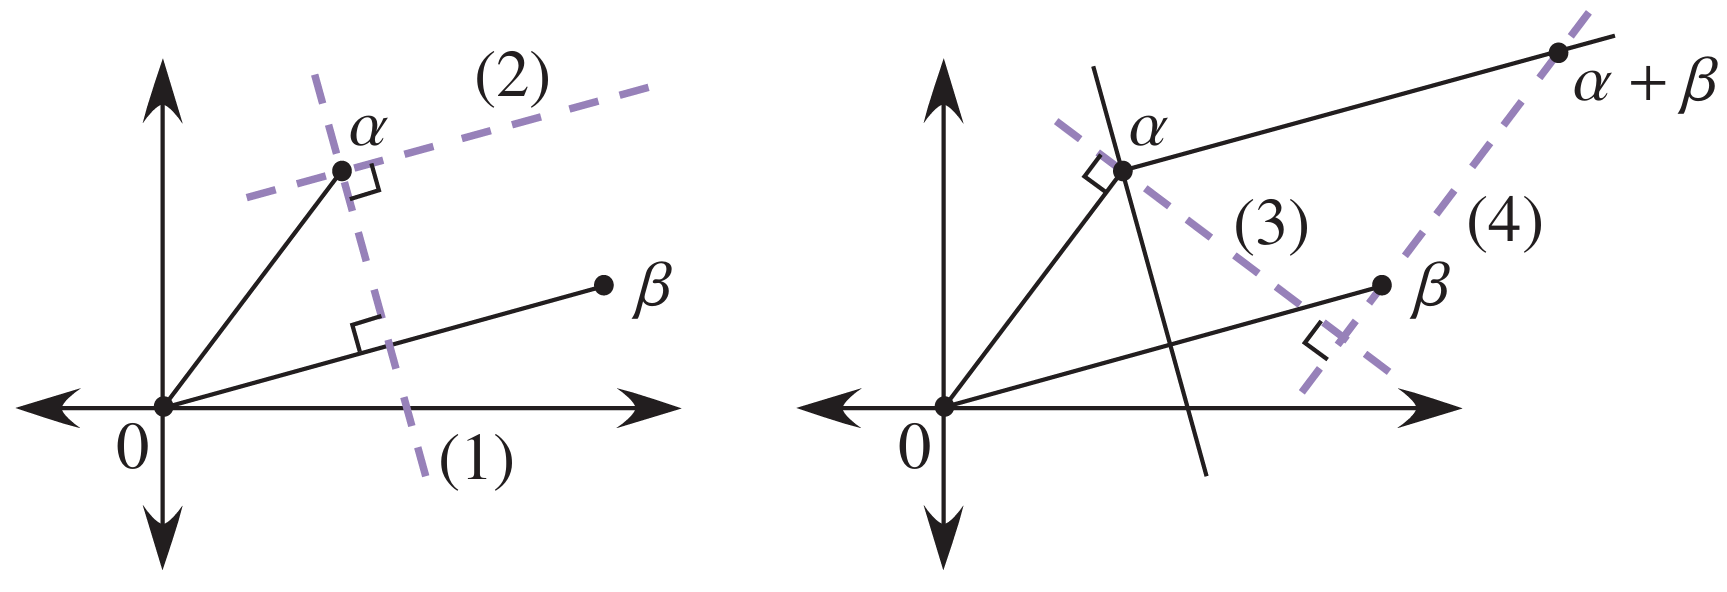
\includegraphics[width=0.7\textwidth]{images/algebra/sestevanje.png}
        \caption[Seštevanje origami števil]{Konstrukcija števila $\alpha + \beta$.}
        \label{fig:sestevanje}
    \end{figure}

    Za dokaz preostalih dveh zahtev najprej dokažimo, da za neničelna $a, b \in \OR \cap \R$ velja $ab, 1/a \in \OR$, potem pa s pomočjo leme~\ref{trd:zaprt_koord} to dokažemo še za poljubna $\alpha, \beta \in \OR$.

    Naj bosta $a, b \in \OR \cap \R$ poljubna in neničelna (če je katerikoli od njiju enak $0$, je produkt ničeln in že po definiciji origami število). Ker sta $a$ in $b$ origami števili, ju lahko konstruiramo. Naj $b$ leži na realni osi, $ai$ pa na imaginarni (slika~\ref{fig:mnozenje_deljenje} levo). Z dvakratno uporabo operacije~\ref{op:O5} konstruiramo origami število $1 + ai$ (točka $B$). Konstruiramo pregib skozi $O$ in $B$ (premica z naklonom $a$) ter v presečišču s pravokotnico skozi $b$ dobimo število $b + abi$ (točka $C$). Pravokotnica skozi $C$ na imaginarno os na njej konstruira origami število $ab$.

    \begin{figure}[h]
        \centering
        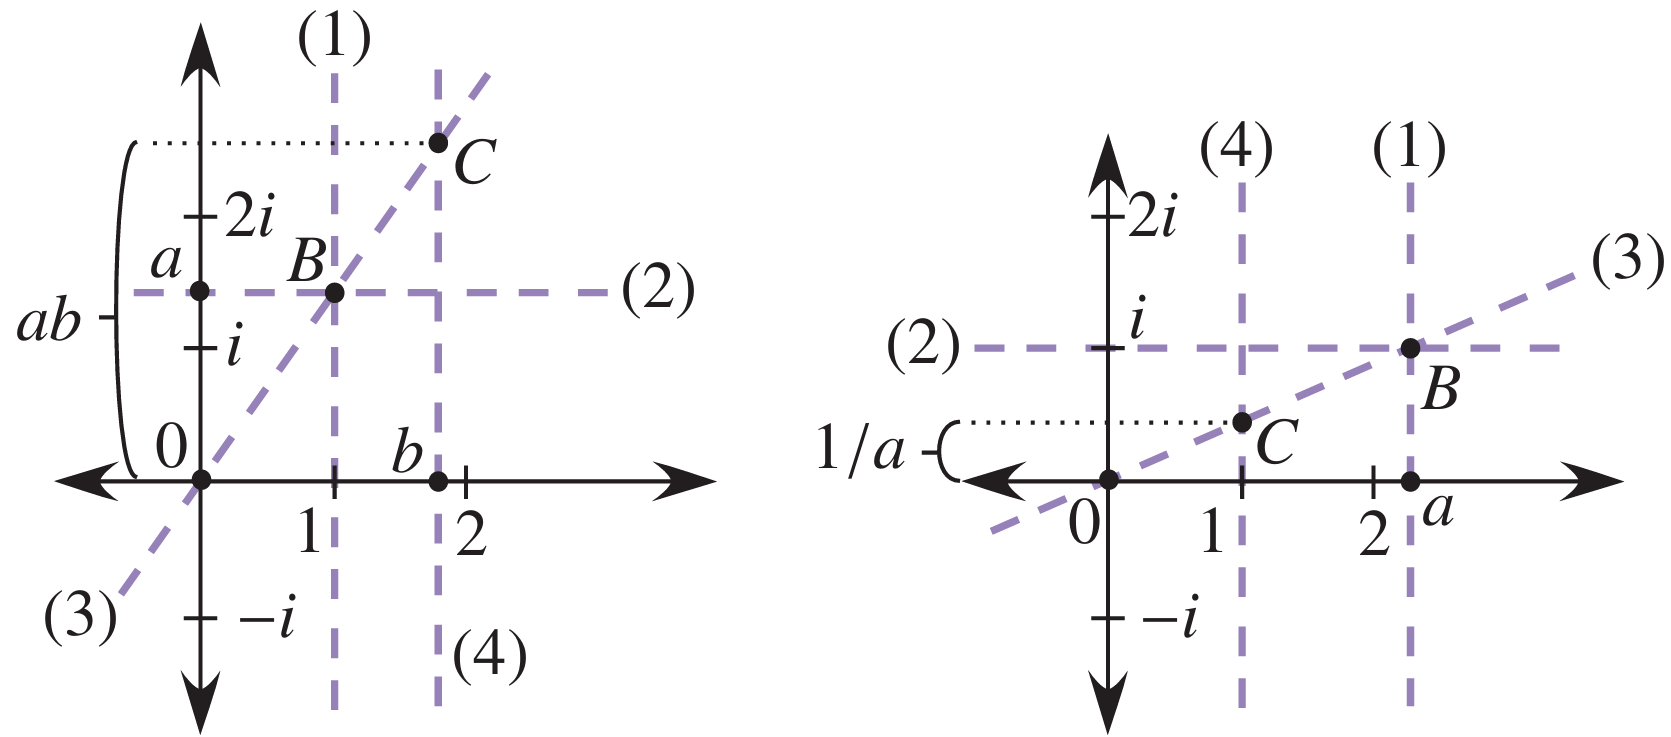
\includegraphics[width=0.7\textwidth]{images/algebra/mnozenje_deljenje.png}
        \caption[Množenje in obratna vrednost realnih origami števil]{Konstrukcija števil $ab$ in $1/a$ za neničelna $a, b \in \OR \cap \R$.}
        \label{fig:mnozenje_deljenje}
    \end{figure}

    Podobno konstruiramo še število $1/a$. Na realni osi konstruiramo število $a$ (slika~\ref{fig:mnozenje_deljenje} desno), s pomočjo~\ref{op:O5} pa še število $a + i$ (točka $B$). Pregib skozi $O$ in $B$ ima naklon ravno $1/a$. V presečišču tega pregiba s pravokotnico na realno os v točki $1$ dobimo število $1 + (1/a) i$ (točka $C$). Tako nam pravokotnica na imaginarno os skozi točko $C$ konstruira origami število $1/a$.

    Vzemimo sedaj poljubna $\alpha, \beta \in \OR$. Če je $\alpha = a + bi, \beta = c + di$, potem po lemi~\ref{trd:zaprt_koord} velja $a, b, c, d \in \OR$. Število $\alpha \beta = (ac - bd) + (ad + bc)i$ ima v svojem realnem in imaginarnem delu vsote, razlike in produkte origami števil, ki so prav tako origami števila. Torej je $\alpha \beta \in \OR$.

    Za neničeln $\alpha = a + bi \in \OR$ je $1/\alpha = a/(a^2+b^2) + (-b)/(a^2+b^2)i$. Ker sta po lemi~\ref{trd:zaprt_koord} števili $a, b \in \OR$, sta zopet realni in imaginarni del tega števila origami števili, torej $1/\alpha \in \OR$.
\end{dokaz}

\begin{trditev}
    \label{trd:zaprtost_koren}
    Naj bo $\alpha \in \OR$. Potem velja $\sqrt{\alpha}, \sqrt[3]{\alpha} \in \OR$.
\end{trditev}

\begin{dokaz}
    Naj bo $\alpha = r e^{i \theta}$ za neka $r \in (0, \infty)$ (v ničelnem primeru ni kaj dokazovati) in $\theta$ poljuben kot. Torej imamo za kvadratni in kubični koren števila $\alpha$ skupno pet rešitev:
    \begin{itemize}
        \item $\sqrt{\alpha} = \pm \sqrt{r}e^{i \frac{\theta}{2}}$ in
        \item $\sqrt[3]{\alpha}_1 = \sqrt[3]{r}e^{i \frac{\theta}{3}}, \sqrt[3]{\alpha}_2 = \sqrt[3]{r}e^{i \left(\frac{\theta}{3} + \frac{2\pi}{3}\right)}, \sqrt[3]{\alpha}_3 = \sqrt[3]{r}e^{i \left(\frac{\theta}{3} + \frac{4\pi}{3}\right)}$.
    \end{itemize}
    Torej moramo dokazati, da $\sqrt{r}, \sqrt[3]{r} \in \OR$, da znamo razpolavljati in tretjiniti kote ter rotirati origami število za kot $60^\circ$ okoli izhodišča $O$. Potem bomo po izreku~\ref{izr:podpolje} lahko konstruirali zgornjih pet števil in tako dokazali to trditev.

    Najprej se še prepričajmo, da $r \in \OR$. Ker je to ravno razdalja števila $\alpha$ do izhodišča, jo lahko prenesemo na realno os in tako konstruiramo realno število $r$, torej je res $r \in \OR$.

    Za konstrukcijo števila $\sqrt{r}$ vzemimo točko $A = (0, 1) $ in premico $y = -1$. Na ordinatni osi označimo točko $B = (0, -r/4)$ in z operacijo~\ref{op:O6} skoznjo naredimo pregib, ki točko $A$ položi na premico $y = -1$. Njena zrcalna slika je $A'=(t, -1) $ za nek $t \in \R$. Na koncu prepognemo še pravokotnico na abscisno os skozi točko $A'$ in tako dobimo točko $(t, 0)$ (slika~\ref{fig:konstrukcija_korena}).
    \begin{figure}[h]
        \centering
        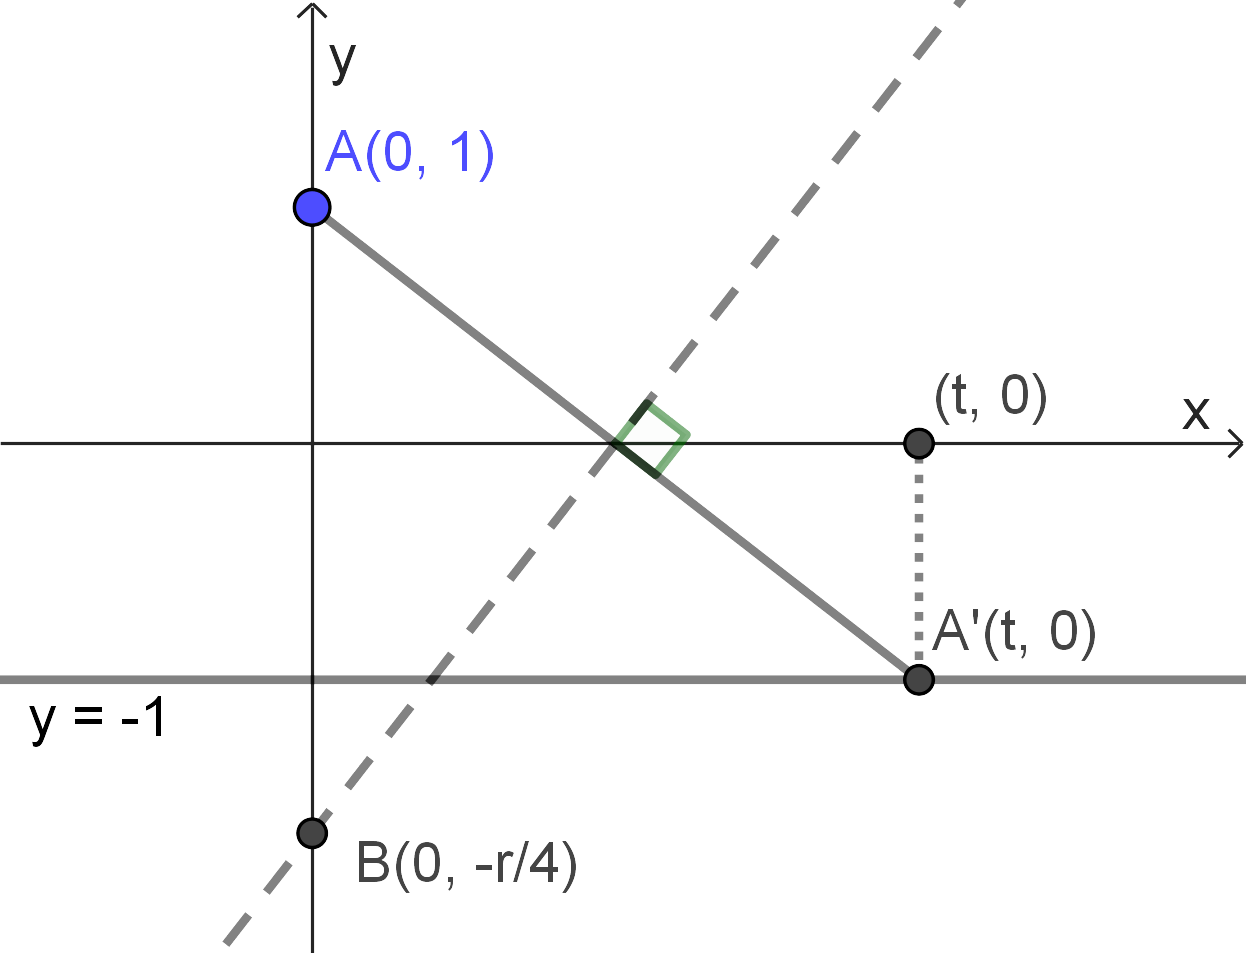
\includegraphics[width=0.5\textwidth]{images/kvadratni_koren.png}
        \caption[Konstrukcija korena]{Konstrukcija števila $\sqrt{r}$ za poljuben $r \in \Q^{+}$.}
        \label{fig:konstrukcija_korena}
    \end{figure}

    Pokažimo, da je $t = \sqrt{r}$. Pregib po konstrukciji poteka skozi točko $B$ in razpolovišče daljice $AA'$, torej je njegov koeficient $k_B = \frac{r}{2t}$ (izpeljavo prepuščamo bralcu). Ker je pregib simetrala daljice $AA'$, njena nosilka pa ima koeficient $k_A = - \frac{2}{t}$, dobimo
    \begin{align*}
        k_B &= - \frac{1}{k_A},\\
        \frac{r}{2t} &= \frac{t}{2},\\
        r &= t^2 \text{ oz. } t = \sqrt{r}.
    \end{align*}    
    V poglavju~\ref{pogl:enacbe} si bomo pogledali, kako z origamijem na več načinov rešujemo poljubne kubične enačbe z racionalnimi koeficienti (npr.\ v razdelku~\ref{podpogl:lill_beloch_postopek} je opisan Belochin postopek preko Lillove metode), torej bomo znali konstruirati tudi rešitve enačbe $x^3 - r = 0$. Konkretne konstrukcije števila $\sqrt[3]{r}$ so opisane tudi v poglavju~\ref{pogl:starogrskiproblemi} (glej trditev~\ref{trd:koren_3_k}).
    
    Z operacijo~\ref{op:O4} znamo razpoloviti kot, postopek tretjinjenja kota pa je, kot že omenjeno, opisan v razdelku~\ref{podpogl:trisekcija}. Ostane nam samo še rotacija točke za kot $60^\circ$ okoli izhodišča. Na sliki~\ref{fig:kot60_rotacija} je prikaz enostavne konstrukcije -- najprej prepognemo simetralo $p_1$ daljice $OA$ in konstruiramo pregib $p_2$ skozi $O$, ki točko $A$ preslika v točko $A'$ na simetrali $p_1$. Trikotnik $\triangle OAA'$ je enakostraničen. 
    \begin{figure}[h]
        \centering
        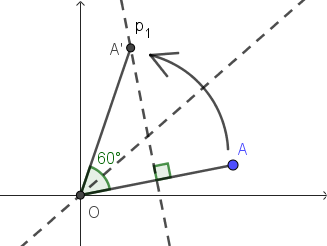
\includegraphics[width=0.4\textwidth]{images/algebra/kot60.png}
        \caption[Rotacija točke okoli izhodišča]{Rotacija točke za kot $60^\circ$ okoli izhodišča.}
        \label{fig:kot60_rotacija}
    \end{figure}
\end{dokaz}

Množica origami števil $\OR$ je tako podobseg kompleksnih števil, ki vsebuje racionalna števila in je zaprt za seštevanje, odštevanje, množenje, deljenje ter za kvadratno in kubično korenjenje. Z origamijem znamo zrcaliti točke, zato je očitno zaprta tudi za konjugiranje. Z njim tako lahko poleg kvadratnih rešujemo tudi poljubne kubične enačbe (izračun rešitev po Cardanovi formuli ne potrebuje več kot ravno naštete operacije), a s tem se bomo natančneje ukvarjali v poglavju~\ref{pogl:enacbe}.
% \begin{posledica}
%     Množica origami števil $\OR$ je %najmanjši
%     podobseg polja $\C$, ki vsebuje racionalna števila in je zaprt za kvadratno in kubično korenjenje ter kompleksno konjugiranje.
% \end{posledica}
Na množici $\OR$ torej lahko uporabimo vse tiste operacije, ki jih lahko izvajamo na množici evklidsko-konstruktibilnih števil; ker pa lahko origami števila tudi kubično korenimo, je origami števil še več (vemo že na primer, da število $\sqrt[3]{2}$ ni evklidsko-konstruktibilno, je pa origami število).

\begin{posledica}
    Množica evklidsko-konstruktibilnih števil je prava podmnožica množice origami števil.
\end{posledica}

Kaj je naša množica origami števil? Po zgledu posledice~\ref{posl:podmnozice} očitno velja $\Q \subset \OR \subset \C$. Kot pri evklidsko-konstruktibilnih številih bomo tudi tu iskali razširitve polja racionalnih števil, ki so zaprte za operacijo kvadratnega korena, za razliko od prej pa tu dodamo še zaprtost za operacijo kubičnega korena.

Znamo konstruirati kompleksno število $i$. Naj bo $\Q(i)$ razširitev polja $\Q$, tj.\ $\Q \subset \Q(i)$ in velja $[\Q(i) : \Q] = 2$, saj je $x^2 + 1$ minimalni polinom števila $i$ nad $\Q$. Polje nadalje razširimo z origami številom $\sqrt[3]{2}$. Dobimo zaporedje $\Q \subset \Q(i) \subset \Q(i, \sqrt[3]{2})$ in velja $[\Q(i, \sqrt[3]{2}) : \Q(i)] = 3$, saj je $x^3 - 2$ minimalni polinom števila $\sqrt[3]{2}$ nad $\Q(i)$.

\begin{definicija}
    Naj bosta $E \subset F$ polji. Če velja $[F:E] \in \{2,3\}$, polju $F$ pravimo \emph{$2,3$-razširitev} polja $E$.
\end{definicija}

Pred naslednjim izrekom poglejmo še lemo, pri čemer za kratek čas zapustimo množico kompleksnih števil in se vrnimo v realno ravnino.

\begin{lema}
    \label{lema:O7_razširitev}
    Naj bosta $A$ in $B$ točki s koordinatama iz polja $E$ ter premici $a$ in $b$, kjer so koeficienti iz njunih implicitnih enačb prav tako elementi polja $E$. Opravimo Belochin pregib, ki točko $A$ preslika na premico $a$ ter točko $B$ na premico $b$. Premica, ki pripada pregibu, ima potem koeficiente iz razširitve polja $E$, ki je stopnje največ $3$.
\end{lema}
\begin{dokaz}
    Najprej obravnavajmo primer, ko točki ne ležita na nobeni izmed premic. Brez škode za splošnost vzemimo $A = (0,1)$ in $a : y = -1$. Naj bo $B = (x_0, y_0)$ in $b : a_1 x + b_1 y = c_1$, kjer so $x_0, y_0, a_1, b_1, c_1 \in E$.

    Analogno kot pri konstrukciji števila $\sqrt{r}$ (glej dokaz trditve~\ref{trd:zaprtost_koren}) nam tu Belochin pregib točko $A$ preslika v točko $A' = (t, -1)$ za nek $t$. Enačba pregiba je tako
    \begin{equation}
        \label{eq:en_pregiba}
        y = \frac{t}{2}x - \frac{t^2}{4}.
    \end{equation}
    Naš cilj je dokazati obstoj razširitve $F$ polja $E$, da je $t \in F$ in velja $[F:E] \leq 3$. Naj bo $B' = (x_1, y_1)$ zrcalna slika točke $B$ preko Belochinega pregiba. Daljici $AA'$ in $BB'$ sta vzporedni, zato nam enačenje koeficientov njunih nosilk da zvezo
    \begin{equation}
        \label{eq:enaka_koef}
        -\frac{2}{t} = \frac{y_1 - y_0}{x_1 - x_0}.
    \end{equation}
    Upoštevamo, da središče daljice $BB'$ s koordinatama $((x_0 + x_1)/2, (y_0 + y_1)/2)$ leži na premici z enačbo~\ref{eq:en_pregiba} in nato iz zveze~\ref{eq:enaka_koef} izrazimo koordinati $x_1$ in $y_1$ (računsko izpeljavo prepuščamo bralcu). Dobimo parametrizacijo krivulje, ki jo opiše točka $B'$ preko različnih pregibov, ki točko $A$ položijo na premico $a$. Ko upoštevamo še, da točka $B'$ leži na premici $b$, dobimo \emph{kubično} enačbo za parameter $t$, ki ima vse koeficiente izražene s števili $x_0, y_0, a_1, b_1$ in $c_1$. Zato je dovolj, da je stopnja razširitve polja $E$, ki vsebuje število $t$, največ $3$.

    Obravnavajmo še primer, ko ena ali obe izmed točk $A$ in $B$ ležita na premicah $a$ in $b$. Iz izreka~\ref{izr:dve_operaciji} vemo, da je izveden Belochin pregib v resnici ena izmed operacij~\ref{op:01}, \ref{op:O3}--\ref{op:O6} in~\ref{op:O8}. Bralcu prepuščamo daljši računski premislek po zgledu iz prvega dela dokaza, da za vsako izmed teh operacij in pri vsaki izbiri dveh točk in premic rešujemo enačbo največ druge stopnje.
\end{dokaz}

\begin{izrek}
    \label{izr:orig_konstr}
    Število $\alpha \in \C$ se da konstruirati le s prepogibanjem papirja natanko tedaj, ko obstaja zaporedje $2,3$-razširitev polja $\Q$ oblike
    $$ \Q = F_0 \subset F_1 \subset F_2 \ldots \subset F_{n-1} \subset F_n \subset \C $$
    za nek $n \in \N_0$, da je $\alpha \in F_n$.
\end{izrek}

\begin{dokaz}
    Naj bo $ \Q = F_0 \subset F_1 \subset F_2 \ldots \subset F_{n-1} \subset F_n \subset \C $ zaporedje $2,3$-razširitev polja $\Q$. Z indukcijo dokažimo $F_n \subset \OR$. Za $n = 0$ je to očitno ($\Q \subset \OR$). Recimo, da velja $F_{n-1} \subset \OR$. Naj bo $f$ minimalni polinom števila $\alpha \in F_n$ nad poljem $F_{n-1}$, ki je stopnje največ $3$, saj velja $[F_n : F_{n-1}] \in \{2,3\}$. Število $\alpha$ je ničla tega polinoma, zato ga dobimo preko reševanja enačbe druge ali tretje stopnje, kar pa z origamijem znamo (glej poglavje~\ref{pogl:enacbe}). Zato je $\alpha \in \OR$.

    Naj bo sedaj $\alpha = a+bi \in \OR$. Želimo konstruirati zaporedje $2,3$-razširitev $\Q = F_0 \subset \ldots \subset F_n$, da bo veljalo $a, b \in F_n$. Iz tega bo sledilo $\alpha \in F_n(i)$, ki je stopnje razširitve $2$ in nam dopolni iskano zaporedje razširitev polja $\Q$.

    Po izreku~\ref{izr:dve_operaciji} vemo, da lahko kakršnokoli origami konstrukcijo opravimo z operacijama~\ref{op:O2} in~\ref{op:O7}. Z indukcijo na številu $N$ uporabe operacije~\ref{op:O2} na konstrukciji števila $\alpha$ poiščimo zaporedje $2,3$-razširitev.

    Operacija~\ref{op:O2} nam določi novo origami konstruktibilno točko oz.\ origami število kot presečišče dveh premic. Za $N = 0$ nismo konstruirali nove točke, torej je $\alpha$ že dano število in je $\Q = F_0 \subset \C$ naša $2,3$-razširitev. Recimo sedaj, da za vsako konstrukcijo origami števila preko končnega števila uporabe operacij~\ref{op:O2} ali~\ref{op:O7}, od česar se operacije~\ref{op:O2} poslužimo $(N-1)$-krat, obstaja končno zaporedje $2,3$-razširitev obsega $\Q$.
    
    Naj bo $M$ število uporabe operacij~\ref{op:O2} ali~\ref{op:O7} za konstrukcijo števila $\alpha$, pri čemer smo operacijo~\ref{op:O2} uporabili $N$-krat. V konstrukciji števila $\alpha$ je to očitno zadnja izvedena operacija, saj je število $\alpha$ določeno kot točka v ravnini. Naj bo $\alpha$ presečišče origami-konstruktibilnih premic $p_1$ in $p_2$. Obe premici sta bili lahko konstruirani le z operacijo~\ref{op:O7}, torej za vsako od njiju obstajata točki $\alpha_i$ in $\beta_i$, kjer je $i \in \{1,2\}$, ter še po dve premici, da je $p_i$ njihov ustrezen Belochin pregib. Števila $\alpha_1, \beta_1, \alpha_2, \beta_2$ so bila konstruirana iz največ $(N-1)$-kratne uporabe uperacije~\ref{op:O2}, torej obstaja zaporedje $2,3$-razširitev polja $\Q$ oblike $\Q = F_0 \subset \ldots \subset F_n$, da so realni in imaginarni deli teh štirih števil vsebovani v $F_n$.
    
    Polje $F_n$ razširimo s poljem $F_{n+1}$, ki vsebuje koeficiente premic $p_1$ in $p_2$. Po lemi~\ref{lema:O7_razširitev} je potem $[F_{n+1}:F_n] \leq 3$. Presečišče Belochinih pregibov $p_1$ in $p_2$, ki je naše število $\alpha$, se izračuna iz linearne enačbe s koeficienti iz $F_n$, torej bo veljalo $\alpha \in F_{n+1}$.
\end{dokaz}

Iz tega izreka sledi končna klasifikacija origami števil.

\begin{definicija}
    Naj bo $F$ razširitev polja $E$. Pravimo, da polinom $f(X) \in E[X]$ \emph{razpade} v $F$, če je $f(X)$ enak produktu linearnih polinomov iz $F[X]$. Če $f(X)$ razpade v $F$ in v nobenem drugem podpolju polja $F$, ki vsebuje $E$, potem polju $F$ pravimo \emph{razpadno polje} polinoma $f(X)$ nad poljem $E$.
\end{definicija}

\begin{izrek}
    \label{izr:orig_razp_polje}
    Naj bo število $\alpha \in \C$ algebraično nad poljem $\Q$ in naj bo $L$ razpadno polje minimalnega polinoma števila $\alpha$ nad $\Q$. Potem je $\alpha$ origami število natanko takrat, ko velja $[L:Q]=2^a3^b$ za neka $a, b \in \N_0$.
\end{izrek}
\begin{dokaz}
    Naj bo $\alpha \in \OR$ poljubno origami število. Polje origami števil $\OR$ je zaprto za kvadratne in kubične korene (gl.\ trditev~\ref{trd:zaprtost_koren}), origami operacije~\ref{op:O1}--\ref{op:O8} pa generirajo števila, ki so rešitve polinomov iz $\Q[X]$ stopnje $3$ ali manj (gl.\ dokaz leme~\ref{lema:O7_razširitev}). Zaradi obstoja formul za rešitve kvadratnih in kubičnih enačb polje $\OR$ vsebuje vse rešitve polinomov iz $\Q[X]$ stopnje največ 3. Vsak polinom nad $\Q$ stopnje največ $3$ torej razpade v polju $\OR$, zato je mnnožica origami števil razpadno polje minimalnega polinoma števila $\alpha$ nad poljem $\Q$.
    
    Iz tega sledi $L \subseteq \OR$. Po izreku~\ref{izr:orig_konstr} obstaja zaporedje $2,3$-razširitev oblike $ \Q = F_0 \subset F_1 \subset F_2 \ldots \subset F_{n-1} \subset F_n = L \subset \C $. Kot v dokazu posledice~\ref{posl:kvadr_razs} lahko tudi tu dokažemo, da potem velja $[L:\Q]=2^a3^b$ za neka $a, b \in \N_0$.

    Za dokaz obrata je potrebno nekaj znanja Galoisove teorije. Za Gloisovo grupo Gal$(L/ \Q)$ velja $|$Gal$(L/ \Q)| = [L:\Q] = 2^m3^n$, kar pomeni, da je taka grupa rešljiva (glej~\cite{burnside1904}). Iz tega se lahko zgradi zaporedje $2,3$-razširitev polja $\Q$ za število $\alpha$, ki je po izreku~\ref{izr:orig_konstr} zato origami število.
\end{dokaz}

Origami števila so torej vsa števila, ki jih lahko iz danih kompleksnih števil $0$ in $1$ dobimo s končnim številom uporabe uperacij seštevanja, odštevanja, množenja, deljenja, konjugiranja, kvadratnega ter kubičnega korenjenja. Z njimi lahko posledično rešujemo kvadratne in kubične enačbe. Kako pa je s konstrukcijo kakšnih posebnih geometrijskih oblik, kot so pravilni večkotniki?

\subsubsection{Origami-konstruktibilnost pravilnih $n$-kotnikov}
\label{podpogl:n_kotniki}

Iz evklidske geometrije vemo, za katere $n$ lahko z evklidskim orodjem konstruiramo pravilni $n$-kotnik. Spodnjega izreka tako ne bomo dokazali, ga pa bomo razširili na origami konstrukcije.

\begin{definicija}
    Praštevilo $p$ se imenuje \emph{Fermatovo praštevilo}, če je oblike $p = 2^{2^m} + 1$ kjer je $m \in \N_0$.
\end{definicija}
Prvih nekaj Fermatovih praštevil\footnote{Fermat je domneval, da je vsako število oblike $2^{2^s} + 1$ praštevilo. To pa ni res. Že Euler je ugotovil, da je število $2^{2^5} + 1$ sestavljeno. Deljivo je s številom 641.} je (zaporedje $A000215$ v OEIS -- \emph{On-Line Encyclopedia of Integer Sequences}):
$$3,\; 5,\; 17,\; 257,\; 65537,\; 4294967297,\; 18446744073709551617, \ldots $$

\begin{izrek}[Gauss-Wantzelov izrek]
    Pravilni $n$-kotnik se lahko konstruira z neoznačenim ravnilom in šestilom natanko takrat, ko je $n = 2^a p_1 \cdots p_k$ za neka $a,k \in \N_0$, kjer so $p_1, \ldots, p_k$ različna Fermatova praštevila.
\end{izrek}

Za $n \leq 20$ pravilni $n$-kotnik \emph{ni} evklidsko-konstruktibilen v primeru
$$n \in \{ 7,\;9,\;11,\;13,\;14,\;18,\;19 \}.$$

Za origami-konstruktibilnost pravilnega večkotnika se namesto Fermatovih praštevil poslužimo pomnožice praštevil, ki sta jo definirala Cox in Shurman v~\cite{cox2005}.

\begin{definicija}
    Praštevilo $p$ se imenuje \emph{Pierpontovo\footnote{Ameriški matematik James Pierpont (1866--1938) je ta praštevila uvedel l.\ 1895, ko je opisoval, katere pravilne večkotnike lahko konstruiramo preko stožnic.
    %Izkaže se, da so origami konstrukcije natanko konstrukcije preko stožnic in obratno.
    } praštevilo}, če je $p > 3$ in $p = 2^m3^n + 1$ za neka $m,n \in \N_0$.
\end{definicija}

\begin{izrek}
    Pravilni $n$-kotnik se lahko konstruira z origamijem natanko takrat, ko je $n = 2^a 3^b p_1 \cdots p_k$ za neke $a,b,k \in \N_0$, kjer so $p_1, \ldots, p_k$ različna Pierpontova praštevila.
\end{izrek}
\begin{dokaz}
    Naj bo $\zeta_n = e^{2 \pi i / n}$ $n$-ti koren enote. Pravilni $n$-kotnik lahko konstruiramo, če in samo če lahko konstruiramo kot $2 \pi / n$, kar je ekvivalentno obstoju konstrukcije števila $\zeta_n$. To število je ničla polinoma $z^n - 1 \in \Q[z]$, katerega razpadno polje je $\Q(\zeta)$. Po izreku~\ref{izr:orig_razp_polje} je $\zeta_n \in \OR$ natanko takrat, ko je $[\Q(\zeta_n) : \Q] = 2^a3^b$ za neka $a, b \in \N_0$.

    Minimalni polinoma števila $\zeta_n$ nad $\Q$ je oblike
    $$ \Phi_n(z) = \prod_{\substack{0 \leq i < n, \\ \gcd(i,n)=1}} (z - \zeta_n^i). $$
    To je dokazano v več matematičnih besedilih, ki govorijo o Galoisovi teoriji, npr.\ v~\cite[poglavje $9.1$]{cox2005}.
    Sledi $[\Q(\zeta_n) : \Q] = \deg(\Phi_n(z)) = \phi(n)$, kjer je $\phi$ Eulerjeva funkcija, ki pove, koliko naravnih števil, manjših od $n$, je tujih številu $n$. Ena od številnih formul za izračun Eulerjeve funkcije je $\phi(n) = n \prod_{p|n} (1 - 1/p)$ za $n \in \N$.

    Naj bo sedaj $n = 2^a 3^b p_1 \cdots p_k$ za neke $m,n,k \in \N_0$, kjer so $p_1, \ldots, p_k$ različna Pierpontova praštevila. Potem je
    \begin{align*}
        [\Q(\zeta_n) : \Q] &= \phi(n) \\
        &= n \prod_{p|n} (1 - \frac{1}{p}) =
        \begin{cases}
            2^a3^{b-1}(p_1 -1) \cdots (p_k -1), &a,b>0,\\
            2^{a-1}(p_1 -1) \cdots (p_k -1), &a>0, b=0,\\
            2 \cdot 3^{b-1}(p_1 -1) \cdots (p_k -1), &a=0,b>0,\\
            (p_1 -1) \cdots (p_k -1), &a=b=0.
            \end{cases}
    \end{align*}
    Torej je $[\Q(\zeta_n) : \Q] = 2^s3^t$ za neka $s,t \in \N_0$, torej je $\zeta_n \in \OR$.

    Za dokaz obrata predpostavimo $\zeta_n \in \OR$, torej je $[\Q(\zeta_n) : \Q] = \phi(n) = 2^s3^t$ za neka $s,t \in \N_0$. Faktorizirajmo število $n$ v produkt potenc praštevil kot $n = q_1^{a_1} \cdots q_r^{a_r}$. Potem je
    $$ \phi(n) = n \prod_{p|n} (1 - \frac{1}{p}) = q_1^{a_1-1} (q_1 -1) \cdots q_r^{a_r-1} (q_r -1).$$
    Če je kak $q_i$ sod, je lahko le $q_i = 2$. Če je kateri izmed $q_i$ lih, pa je lahko le $q_i = 3$ ali $a_i = 1$. Poleg tega mora biti vsak faktor $(q_i - 1)$ produkt potence števila $2$ s potenco števila $3$, torej je vsak $q_i$, večji od $3$, Piermontovo praštevilo. Tako je vsak prafaktor števila $n$ lahko število $2, 3$ ali Piermontovo praštevilo, s čimer je dokaz zaključen.
\end{dokaz}

Z origamijem sedaj lahko konsturiramo še $7$-, $9$-, $13$-, $14$-, $18$- in $19$-kotnik. Edini $n$-kotnik za $n \leq 20$, ki ni konstruktibilen tako z evklidskim orodjem kot z origamijem, je $11$-kotnik.

\subsubsection*{Konstrukcija pravilnega sedemkotnika}

Najmanjši pravilni večkotnik, ki ga ne moremo konstruirati z evklidskim orodjem, lahko pa ga z origamijem, je torej sedemkotnik. Italijanski matematik Benedetto Scimemi je preko analize sedemkotnika v kompleksni ravnini našel metodo za njegovo konstrukcijo, avstrijski matematik  Robert Geretschläger pa tudi konkretno konstrukcijo. Njune ugotovitve v~\cite{hull2009} lepo povzame Thomas Hull, ki velja za strokovnjaka na področju origamike, in si jih bomo pogledali v nadaljevanju.

Scimemijeva ideja je bila, da si oglišča pravilnega sedemkotnika predstavljamo kot točke na enotski krožnici v kompleksni ravnini, ki ustrezajo sedmemu korenu enote (slika~\ref{fig:7kotnik_kompleksna}), tj.\ tista kompleksna števila $z$, ki rešijo enačbo
\begin{equation}
    \label{eq:7kotnik_basic}
    z^7 - 1 = 0.
\end{equation}
Ena od rešitev je $z=1$, torej eno oglišče leži na realni osi. Preostale rešitve so še
$$ A = e^{\frac{2\pi i}{7}}, \; A^2 = e^{2\frac{2\pi i}{7}}, \; A^3 = e^{3\frac{2\pi i}{7}}, \; A^4 = e^{4\frac{2\pi i}{7}}, \; A^5 = e^{5\frac{2\pi i}{7}} \; \text{ in } \; A^6 = e^{6\frac{2\pi i}{7}}.$$
\begin{figure}[h]
    \centering
    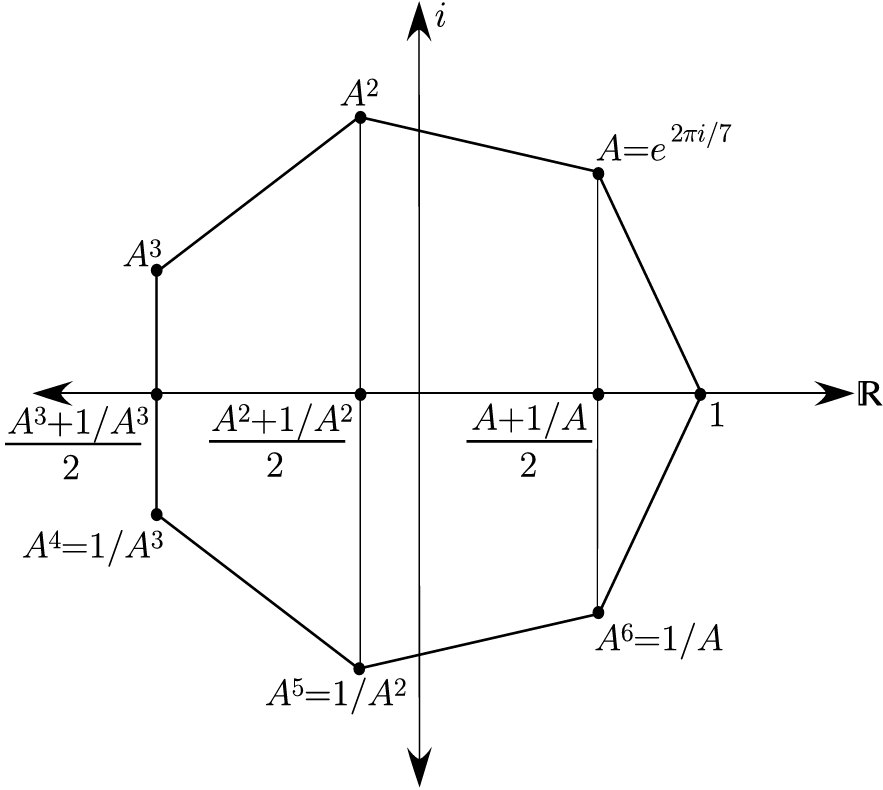
\includegraphics[width=0.6\textwidth]{images/n-kotniki/7kotnik_enotska_kroznica.png}
    \caption[Pravilni sedemkotnik v kompleksni ravnini]{Pravilni sedemkotnik v kompleksni ravnini. Vzeto iz~\cite[str.\ 182]{hull2009}.}
    \label{fig:7kotnik_kompleksna}
\end{figure}

Naš cilj je poiskati metodo, s katero lahko preko prepogibanja papirja konstruiramo kot $2 \pi / 7$, saj znamo rotirati točke za poljuben origami-konstruktibilen kot (točko zrcalimo čez simetralo tega kota).

Sledeča izpeljava je sestavljena iz več korakov. Najprej iz enačbe~\ref{eq:7kotnik_basic} faktoriziramo rešitev $z = 1$ in dobimo enačbo
\begin{equation}
    \label{eq:7kotnik_daljsa_en}
    \frac{z^7-1}{z-1}= z^6+z^5+z^4+z^3+z^2+z+1=0.
\end{equation}
Zaradi simetričnosti sedemkotnika čez realno os lahko to enačbo šeste stopnje preuredimo v enostavnejšo. Ker je $A = e^{2 \pi i / 7} = \cos(2 \pi / 7) + i \sin(2 \pi / 7)$, velja
$$ \frac{1}{A} = \frac{\overline{A}}{A \overline{A}} = \frac{\overline{A}}{\cos^2(2 \pi / 7) + \sin^2(2 \pi / 7)} = \overline{A} = A^6.$$
Ker je $A + 1/A = A + \overline{A} = 2 \cos(2 \pi / 7)$, je središče daljice $A A^6$ ravno točka $(A + 1/A)/2 = \cos(2\pi /7)$ (glej sliko~\ref{fig:7kotnik_kompleksna}).

Iz zveze $1/A = A^6$ sledi še $1/A^2 = A^{12} = A^5$ in $1/A^3 = A^{18} = A^4$. Naj bo $z = A$ in vstavimo ravno izpeljano v enačbo~\ref{eq:7kotnik_daljsa_en}. Dobimo
\begin{equation}
    \label{eq:7kotnik_Aji}
    \frac{1}{A} + \frac{1}{A^2} + \frac{1}{A^3} +A^3+A^2+A+1= 0.
\end{equation}
Razširimo izraza $(A + 1/A)^2$ in $(A + 1/A)^3$ v
$$ A^2 + \frac{1}{A^2} = (A + \frac{1}{A})^2 - 2 \; \text{ in } \; A^3 + \frac{1}{A^3} = (A + \frac{1}{A})^3 - 3(A + \frac{1}{A}),$$
vstavimo to v enačbo~\ref{eq:7kotnik_Aji} in dobimo
\begin{equation*}
    (A + \frac{1}{A})^3 + (A + \frac{1}{A})^2 - 2(A + \frac{1}{A}) - 1 = 0.
\end{equation*}
Torej je $A + 1/A = 2 \cos(2 \pi / 7)$ rešitev enačbe
\begin{equation}
    \label{eq:7kotnik_kubicna}
    z^3 + z^2 - 2z - 1 = 0.
\end{equation}
Podobno bi lahko izpeljali še preostali dve rešitvi te enačbe -- to sta $A^2 + 1/A^2 = 2\cos (4 \pi / 7)$ in $A^3 + 1/A^3 = 2\cos (6 \pi / 7)$, ki sta negativni.

Sedaj iščemo postopek, ki nam konstruira število $2 \cos(2 \pi / 7)$ na realni osi. Iz tega bomo konstruirali pravokotni trikotnik, katerega kot ob izhodišču bo ravno $2 \pi /7$. Nato bomo le še sedemkrat rotirali izbrano točko na realni osi za ta kot okoli izhodišča in s tem konstruirali pravilni sedemkotnik.

Za konstrukcijo števila $2 \cos(2 \pi / 7)$ se bomo poslužili Belochinega pregiba. Vzemimo realno ravnino, na njej pa točki $P_1 = (0,1)$ in $P_2 = (-1, -1/2)$ ter premici $L_1 : y=0$ in $L_2: x=0$. S pregibom položimo točko $P_1$ na abscisno os in hkrati točko $P_2$ na ordinatno os. Njuni sliki zaporedoma označimo s točkama $P'_1 = (t,0)$ in $P'_2 = (0,s)$ za neka $s, t \in \R$, kjer je $t$ očitno pozitiven (slika~\ref{fig:7kotnik_pregib}).

\begin{figure}[h]
    \centering
    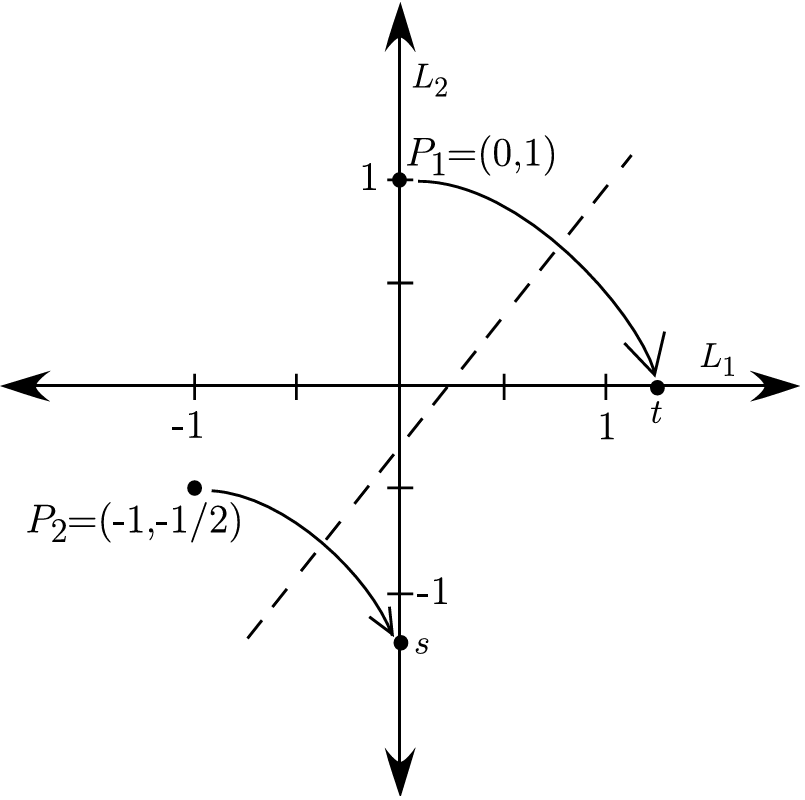
\includegraphics[width=0.45\textwidth]{images/n-kotniki/7kotnik_pregib.png}
    \caption[Pregib za konstrukcijo sedemkotnika]{Pregib za konstrukcijo števila $t = 2 \cos(2 \pi / 7)$. Vzeto iz~\cite[str.\ 184]{hull2009}.}
    \label{fig:7kotnik_pregib}
\end{figure}

Izrazimo enačbo pregiba s spremenljivkama $s$ in $t$. Pregib je pravokoten na daljici $P_1 P'_1$ in $P_2 P'_2$, iz česar dobimo koeficient premice, na koncu pa njeni enačbi (lahka izpeljava je prepuščena bralcu):
\begin{equation*}
    y = tx - \frac{t^2}{2} + \frac{1}{2} \; \text{ in } \; y = -\frac{2}{2s+1}x - \frac{1}{2s+1} + \frac{2s-1}{4}.
\end{equation*}
Ker gre za dve enačbi za isto premico, z enačenjem njunih koeficientov in začetnih vrednosti dobimo sistem dveh enačb za $s$ in $t$:
\begin{equation*}
    t = - \frac{2}{2s+1} \; \text{ in } \; - \frac{t^2}{2} + \frac{1}{2} = - \frac{1}{2s+1} + \frac{2s-1}{4}.
\end{equation*}
Iz prve enačbe izrazimo spremenljivko $s$, jo vstavimo v drugo enačbo in dobimo
\begin{equation*}
    - \frac{t^2}{2} + \frac{1}{2} = \frac{t}{2} + \frac{-\frac{2}{t}-2}{4} \Rightarrow t^3 + t^2 - 2t - 1 = 0.
\end{equation*}
Dobimo ravno enačbo~\ref{eq:7kotnik_kubicna}. Vrednost $t$ je torej njena edina pozitivna rešitev, tj.\ $t = 2 \cos(2 \pi / 7)$. Iz tega samo še konstruiramo pravokotni trikotnik, ki ima oglišči ene katete v $P'_1$ in koordinatnem izhodišču, druga kateta je pravokotna na $x$-os v točki $P'_1$ in hipotenuza ima dolžino $2$. S tem bo kot ob koordinatnem izhodišču ravno $2 \pi /7$ (slika~\ref{fig:7kotnik_kot}).

\begin{figure}[h]
    \centering
    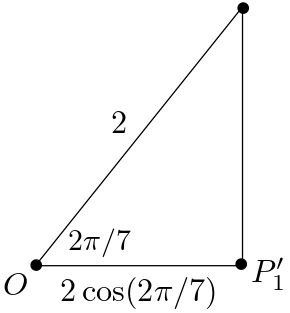
\includegraphics[width=0.25\textwidth]{images/n-kotniki/7kotnik_kot.png}
    \caption[Konstrukcija kota $2 \pi / 7$.]{Konstrukcija kota $2 \pi /7$ preko pravokotnega trikotnika.}
    \label{fig:7kotnik_kot}
\end{figure}

Preostane nam le še navedba konkretne konstrukcije pravilnega sedemkotnika. V ta namen vzemimo v roke kvadraten list papirja, ki predstavlja realno ravnino, in opravimo sledeče korake (gl.\ sliki~\ref{fig:7kotnik_knstr1} in~\ref{fig:7kotnik_knstr2}):
\begin{enumerate}
    \item Predpostavimo, da je stranica kvadrata dolga $4$ enote in je koordinatno izhodišče $O$ v središču kvadrata. Papir dvakrat prepognemo na pol po dolžini, da dobimo obe koordinatni osi, konstruiramo pa še točki $P_1 = (0,1)$ in $P_2 = (-1, -1/2)$.
    \item Opravimo Belochin pregib, ki točko $P_1$ položi na $x$-os in hkrati točko $P_2$ na $y$-os. Sliko točke $P_1$ označimo s $P'_1$.
    \item Konstruiramo pravokotnico na $x$-os skozi točko $P'_1$. Označimo prvo oglišče našega sedemkotnika s točko $B = (2,0)$.
    \item Opravimo prepogib skozi koordinatno izhodišče, ki točko $B$ položi na pravokotnico iz prejšnjega koraka. Sliko točke $B$ označimo z $A$ in predstavlja drugo oglišče sedemkotnika (ker je $|OP'_1| = 2 \cos (2 \pi / 7)$ in $|OA| = 2$).
\begin{figure}[h]
    \centering
    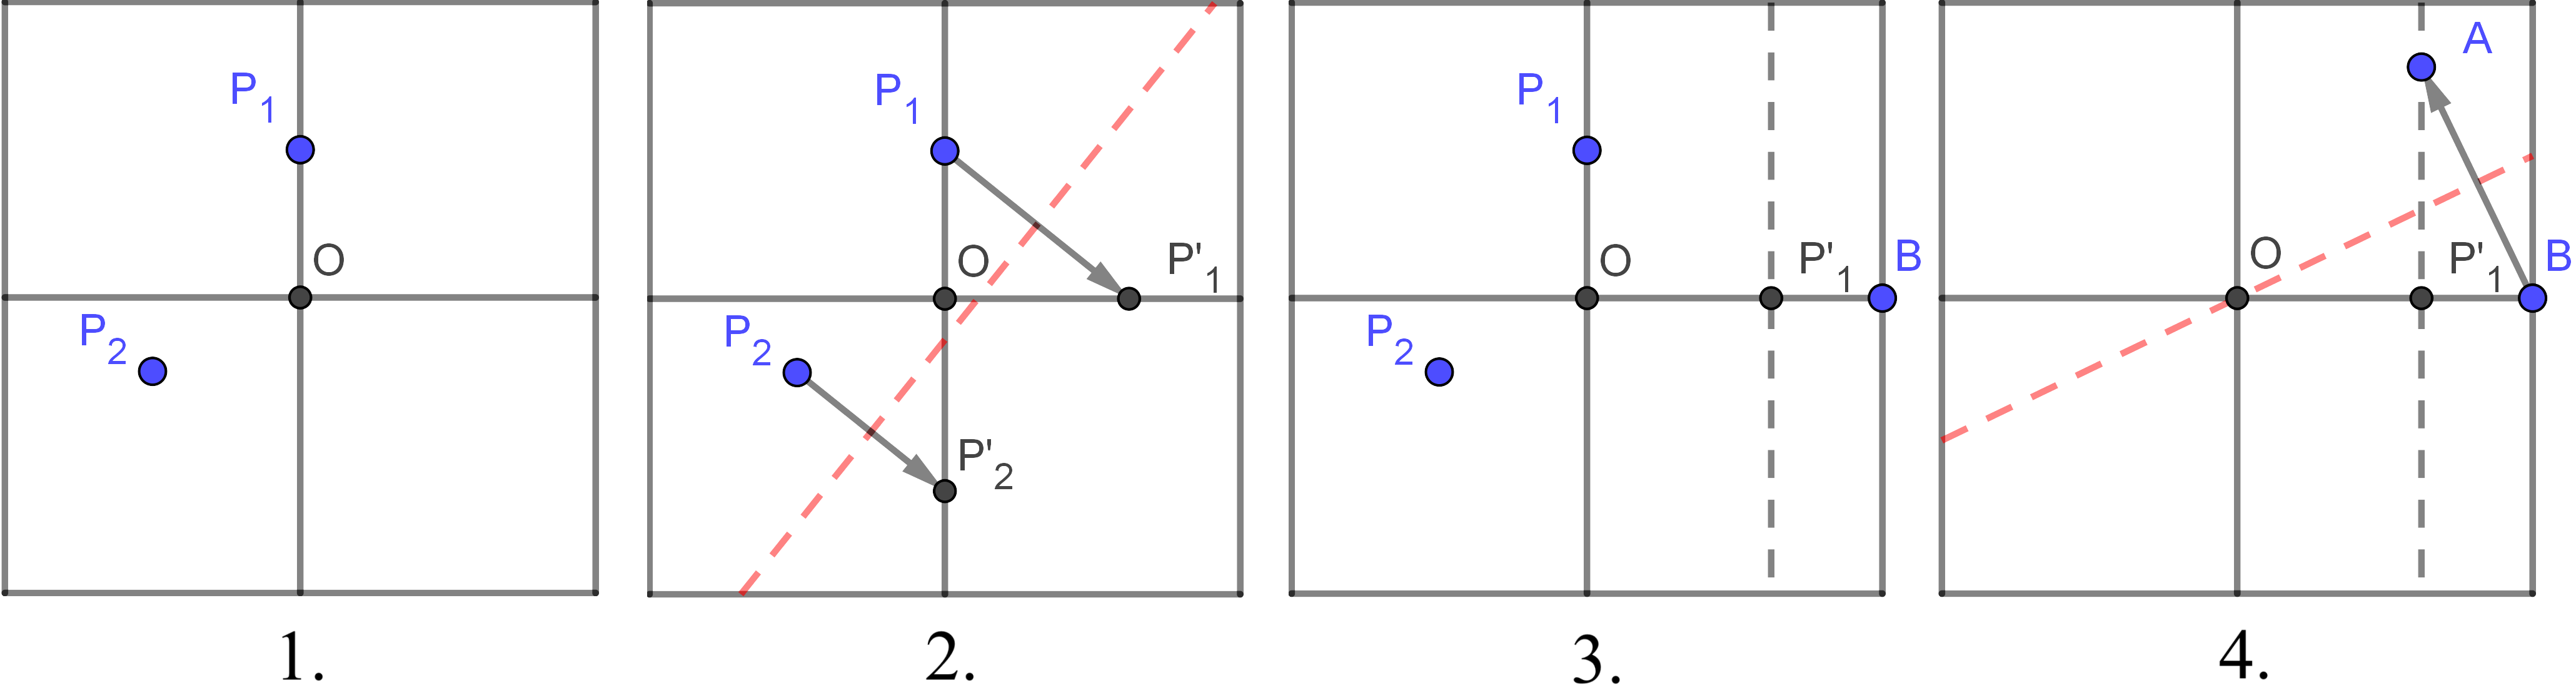
\includegraphics[width=\textwidth]{images/n-kotniki/7kotnik_konstr1.png}
    \caption[Konstrukcija pravilnega sedemkotnika $1$.]{Konstrukcija oglišča $A$ pravilnega sedemkotnika (koraki $1$--$4$).}
    \label{fig:7kotnik_knstr1}
\end{figure}
    \item Korak $4$ opravimo še na spodnjo stran $x$-osi in dobimo točko $A^6$.
    \item Naredimo pregib skozi izhodišče $O$ in točko $A$. Točki $B$ in $A^6$ se čezenj prezrcalita v točki $A^2$ in $A^3$.
    \item Korak ponovimo še za pregib skozi izhodišče $O$ in točko $A^3$. Sliki točk $A^2$ in $A$ označimo s $A^4$ in $A^5$.
    \item Po konstrukciji točke $B, \; A, \; A^2, \; A^3, \; A^4, \; A^5$ in $A^6$ tvorijo oglišča pravilnega sedemkotnika.
    \begin{figure}[h]
        \centering
        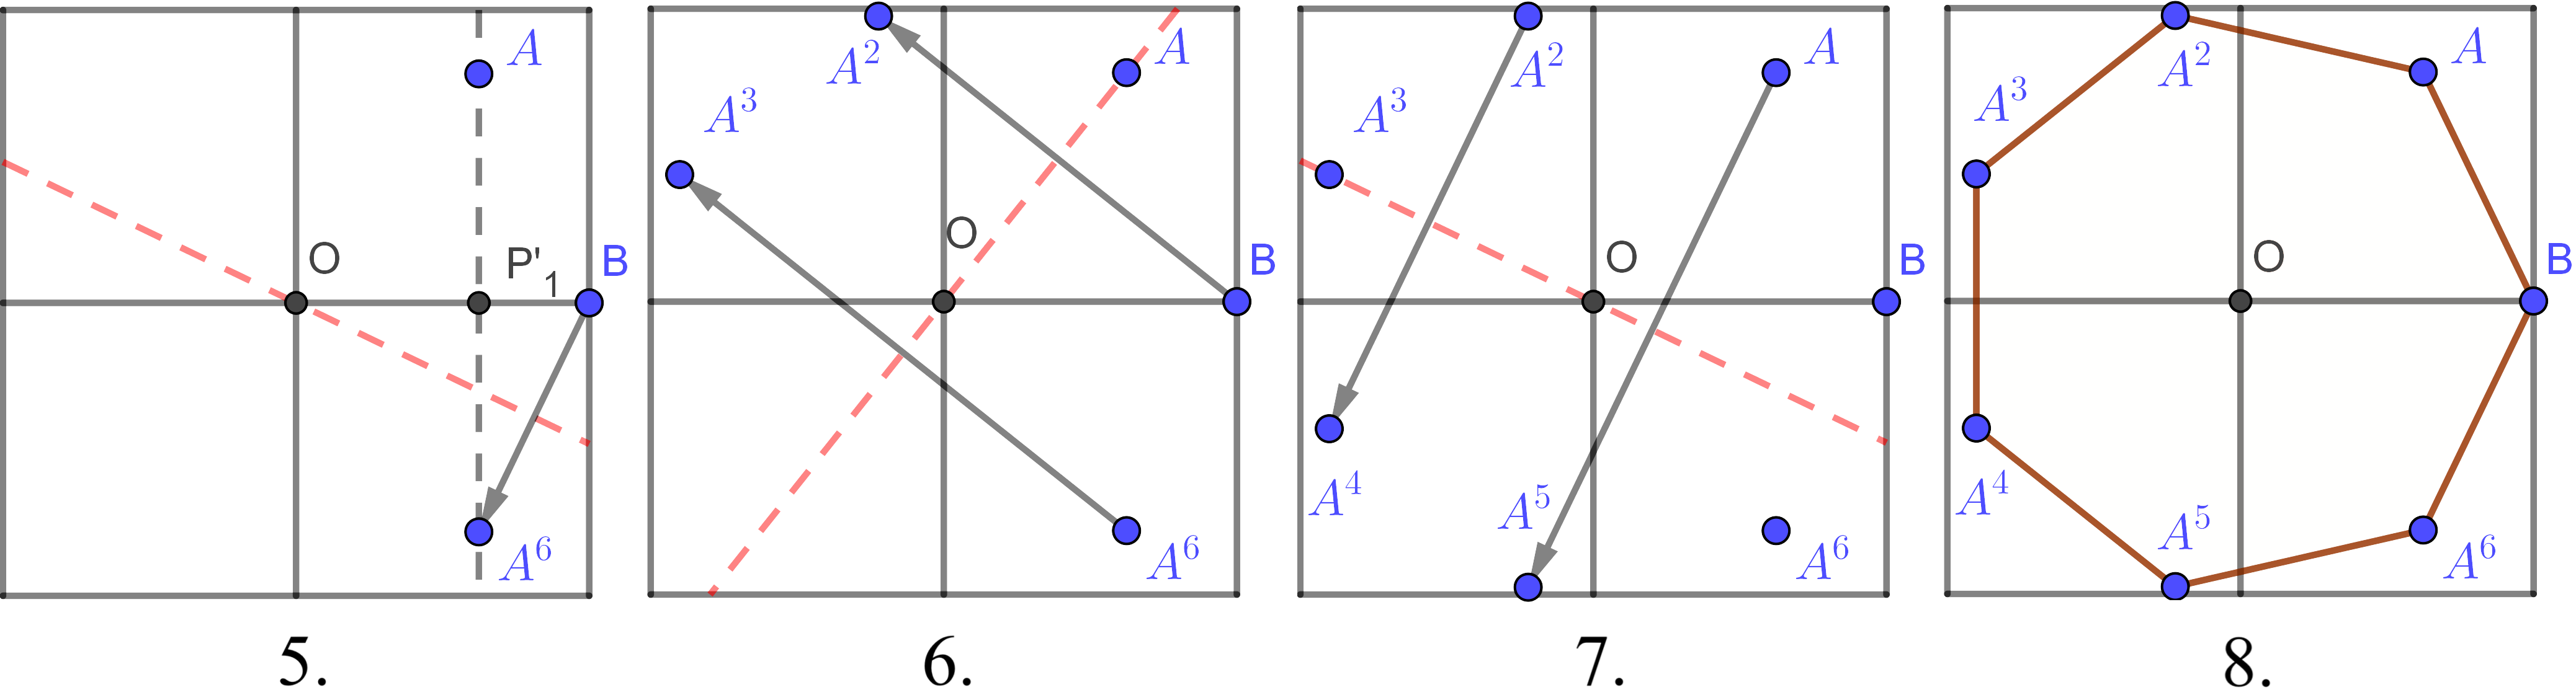
\includegraphics[width=\textwidth]{images/n-kotniki/7kotnik_konstr2.png}
        \caption[Konstrukcija pravilnega sedemkotnika $2$.]{Konstrukcija preostalih oglišč pravilnega sedemkotnika (koraki $5$--$8$).}
        \label{fig:7kotnik_knstr2}
    \end{figure}
\end{enumerate}